\documentclass{report}
\usepackage[utf8]{inputenc}
\usepackage[left = 3cm, top = 3cm, bottom = 3cm, right = 3cm]{geometry}
\usepackage{booktabs}
\usepackage{dsfont}
\usepackage{amsmath, amssymb}
\usepackage{dcolumn}% Align table columns on decimal point
\usepackage{bm}
\usepackage{braket}
\usepackage{graphicx} % Required for inserting images
\usepackage[colorlinks,bookmarks=true,citecolor=blue,linkcolor=red,urlcolor=blue]{hyperref}


\usepackage[
backend=biber,
style=alphabetic,
sorting=ynt
]{biblatex}

\addbibresource{mybibliography.bib}


            
\begin{document}
\begin{titlepage}

\begin{center}
    \LARGE \textbf{Summer Research Fellowship programme (SRFP) Report} \\ \quad \\ \LARGE
    \LARGE \textbf{Indian Academy of Sciences (IAS)} \\ \quad \\ 
    \LARGE \textbf{on} \\ \quad \\ 
    \LARGE\textbf{Topological Phases of Matter}\\
\vspace{1cm}
	\large By	\\ \textbf{Rishi Paresh Joshi } \\ 2nd year, Int. MSc \\National Institute of Science Education and Research(NISER) \\ Bhubaneswar\\[1cm]
 \vspace{1cm}
		 \large Under the supervision of:        \\
		 \large \textbf{ Dr. Ajit C. Balram,} \\
        	Institute of Mathematical Sciences, CIT Campus, Chennai, 600113, India \\
\vspace{1cm}
31/07/2023
\end{center}
\begin{figure}
\centering
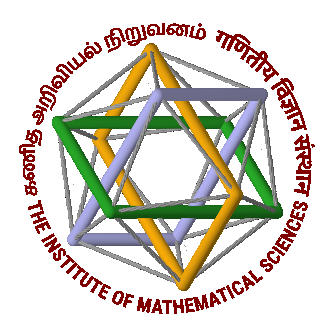
\includegraphics[scale=1]{imsclogo_trilingual_600_new.eps}
\end{figure}

\end{titlepage}



\newpage
\section*{Acknowledgements}
\par I would like to express my sincere gratitude towards my guide, Dr. Ajit C. Balram, for his guidance and expertise throughout the program, which has been invaluable in enhancing my understanding of this fascinating field. This experience has enriched my knowledge and strengthened my passion for research. I thank the Indian Academy of Sciences for this incredible opportunity to explore and learn. Lastly, I would like to thank Rakesh Kumar Dora, Koyena Bose, and Sashikanta Mohapatra, Ph.D. students working with Ajit, for helping me understand the basics of the field.
\newpage
\section{Abstract}
Condensed matter physics deals with phases of matter that exhibit phenomena like superconductivity and quantization of resistivity~\cite{MM}. A phase is a particular organization of particles whose properties are determined by the collective behavior of all the particles in the system. A phase transition occurs when the parameters of the system are changed. Traditionally, phase changes are associated with Landau's theory of symmetry-breaking. However, experiments like the Quantum Hall Effect (QHE) revealed the existence of topological phases where phase transitions occur without symmetry-breaking. In a topological phase, specific properties, such as the Hall conductance or the number of edge modes (equal to Chern number) in a QH system, are independent of material details and insensitive to smooth deformation of the system (such as small density change or disorders) unless the system passes through a quantum phase transition~\cite{J.Moore}. The system's external deformations are considered gentle enough – namely "adiabatic" as long as they are sufficiently smaller than the gap so as not to create excitation above the ground state~\cite{J.Moore}. This report discusses the classical Hall effect, its quantum version, and some of the basics required to understand these.
\newpage
\section{Introduction}
A significant discovery in the 1980s was that electrons, when confined to two dimensions and subject to a strong magnetic field, show a  topological phase that underlies the quantum Hall effect~\cite{J.Moore}. This effect was noticed in the late 1900s as it was impossible to generate low temperatures and high magnetic fields (classically, scattering of electrons rendered the mean free path to decrease, and low   magnetic field increased the radius of the orbit.) Additionally, quantization of resistivity was only first observed in 2DES because, in three dimensions (3D), the Landau levels spread out in energy along the direction of the magnetic field. As a result, no matter where the Fermi energy lies, the Landau levels fill the energy gap and destroy the Hall-resistance plateaus. However, viewing IQHE from the perspective of the Haldane model and the SSH model describing the electric conductivity of polyacetylene gave rise to a new concept of Topological Insulators, which could also be found in 3D~\cite{SSH}~\cite{Haldane}. Before explaining the phenomena of QHE, one can look at the phase at room temperature and low magnetic field through the classical picture involving the Drude model. The various prerequisites required to understand the Quantum phenomena and the basics for other topological phases are covered in this report.
\tableofcontents
\newpage
\chapter{Perturbation theory}
The quantum mechanical study of conservative physical systems is based on the eigenvalue equation of the Hamiltonian operator. The Schrodinger Equation is a second-order differential equation. We may need to find the exact solution to a problem. Two or many-body problems pose such issues. This is because the force on a body is inversely proportional to the square of the distance (the independent variable with respect to which we are differentiating). Thus, even a tiny change in the initial conditions can significantly change the force. Therefore, the system is "chaotic." We still need to solve such equations analytically. If we know the exact solution to the Hamiltonian that excludes a "small" term, then we can use perturbation theory to solve the Hamiltonian, including the "small" term.
\section{What is a perturbation?}
The perturbation is a small action on the system, so its effects can be treated as a series of corrections to the exact solution. A small perturbation is assumed not to change the Hilbert Space of the system on which it acts. The system's state changes such that it can be expressed as a linear combination of the initial state and states orthogonal to the initial state. 

The more the strength of the perturbation, the more will the Hilbert space change. Perturbations that are strong enough that the system leaves its original Hilbert Space are entirely known to cause a phase transition. 

Unitary perturbations don't disturb the Hilbert Space since the inner product of any two vectors is preserved under unitary transformation. An example of this is the interaction of a quantum system with a weak Electromagnetic field. Another critical example is, if given Hilbert Spaces of states for a single particle, we can create a new Hilbert Space of states for two particles by taking a tensor product of their individual Hilbert Spaces. The tensor product is a unitary transformation. Thus, it doesn't affect the states of the individual particles.

\section{General approach}
The Schrodinger Equation is $H\ket{\psi} = E\ket{\psi}$. Assume that we know the exact analytical solution of the eigenvalue problem:\cite{Griffith}
\begin{equation}\label{eq6}
    H^0\ket{\psi_n^0} = E_n^0\ket{\psi_n^0}
\end{equation}
and that we want to find a solution to 
\begin{equation}\label{eq5}
    (H^0+H')\ket{\psi_n} = E_n\ket{\psi_n^0}
\end{equation} 
Using perturbation theory, we can find the approximate solution to eq.\ref{eq5}. However, some conditions must be satisfied for the perturbation theory to give a valid answer. Qualitatively, the condition is that $H'$ should be a "small" perturbation. This is so that the Hilbert space of the initial system, satisfying eq.\ref{eq6}, remains the same even on the addition of the perturbation, i.e., the solution to eq.\ref{eq5} belongs to the same Hilbert Space as spanned by the solutions to eq.\ref{eq6} (for different eigenvalues, E), HS. 

Let's try to solve eq.\ref{eq5} for corresponding to a particular eigenvalue of eq.\ref{eq6}, $E^0$. Thus, we can assume that the corresponding energy eigenvalue and state to be written as 
\begin{align}
    &E_n = E_n^0 + E_n^1 + E_n^2 + ... \\
    &\ket{\psi_n} = \ket{\psi_n^0} + \ket{\psi_n^1} + \ket{\psi_n^2} + ... \in HS
\end{align}

We can treat $\ket{\psi_n^1}$ as a linear combination of orthogonal basis eigenstates of HS. In fact, in the first order approximation, we will see that we can write $\ket{\psi_n^1}$ as a linear combination of orthogonal basis eigenstates of HS, excluding $\ket{\psi_n^0}$. This is because adding any constant multiplied with $\ket{\psi_n^0}$ to $\ket{\psi_n^1}$ will remain a solution until first order correction.

\subsection{First order correction}
In the first-order correction, we define the following:
\begin{align}
    & E_n = E_n^0 + E_n^1 \\ \label{eq7}
    & \ket{\psi_n} = \ket{\psi_n^0} + \ket{\psi_n^1} \in HS \\ \label{eq8}
    & \Rightarrow (H^0 + H')(\ket{\psi_n^0} + \ket{\psi_n^1}) = (E_n^0 + E_n^1)(\ket{\psi_n^0} + \ket{\psi_n^1})
\end{align}
Neglect the terms where a which is a square of the perturbation term or a product of perturbation terms (like the product of $E_n^1$ and $\ket{\psi_n^1}$ and the action of $H$ and $\ket{\psi_n^1}$). Then we get:
\begin{align}
    & (H^0 + H')\ket{\psi_n^0} + H^0 \ket{\psi_n^1} = (E_n^0 + E_n^1)\ket{\psi_n^0} + E_n^0\ket{\psi_n^1} \\
    & \text{From eq. \ref{eq8}}\Rightarrow H'\ket{\psi_n^0} + H^0 \ket{\psi_n^1} = E_n^1\ket{\psi_n^0} + E_n^0\ket{\psi_n^1}\label{eq9}
\end{align}
Let's solve for $E_n^1$. Take the inner product of  eq.\ref{eq9} with $\bra{\psi_n^0}$

\begin{align}
    & \braket{\psi_n^0|H'\psi_n^0}  + \braket{\psi_n^0H^0|\psi_n^1} = E_n^1\braket{\psi_n^0|\psi_n^0} + E_n^0\braket{\psi_n^0|\psi_n^1} \\
    & \Rightarrow \int_{over all space} d^3x_1d^3x_2(\psi_n^{0*} H'\psi_n^0) = E_n^1\label{eq10} \\
    & \Rightarrow E_n = E_n^0 + \int_{over all space} d^3x_1 d^3x_2(\psi_n^{0*} H'\psi_n^0) 
\end{align}

Let's solve for $\ket{\psi_n^1}$. 
\begin{align}
    & \ket{\psi_n^1} = \sum_{j;j \neq n} a_{nj}\ket{\psi_j^0}\label{eq11}
\end{align}
We can see that any constant multiplied with $\ket{\psi_n^0}$ to $\ket{\psi_n^1}$ in eq.\ref{eq11} will remain a  solution to eq.\ref{eq9}, till first order correction. To find $a_{nj}$, take the inner product of  eq.\ref{eq9} with $\bra{\psi_j^0}$

\begin{align}
    & \braket{\psi_j^0|H'\psi_n^0}  + \braket{\psi_j^0|H^0\psi_n^1} = E_n^1\braket{\psi_j^0|\psi_n^0} + E_n^0\braket{\psi_j^0|\psi_n^1} \\
    & \Rightarrow a_{nj} = \frac{(\int_{over all space} d^3x_1d^3x_2(\psi_j^{0*} H'\psi_n^0))}{E_n^- E_j^0} = = \frac{\braket{H'}_{jn}}{E_n^- E_j^0}
\end{align}
\chapter{Identical particles}
\section{What are identical particles?}
Two identical particles have the same intrinsic properties. Intrinsic properties are those of an entity that defines the particle and doesn't change unless the particle changes to another particle~\cite{N.Sneha}. Intrinsic properties include:
\begin{enumerate}
    \item Mass
    \item Charge
    \item Spin
    \item Magnetic moment
    \item Color charge
    \item Lepton number
    \item Baryon number
\end{enumerate}

Identical particles may be in different states. If there are two electrons, one could have a spin-up state, and the other could have a spin-down state, but both are spin-1/2 systems. Thus, they are still identical. Similarly, one Helium atom could have both electrons in the ground state. In contrast, another Helium atom could have one electron in the ground state and another in an excited state. Still, regardless of the energy of the Helium atoms, they are identical~\cite{ProfessorM}. 

\section{Consequence of identical particles}
Let two identical non-interacting particles constitute a physical system. The system remains unchanged under evolution with time and in properties when the roles of the two particles are exchanged. 

In the classical system, we consider the system of n identical particles/ objects to be a part of a more generalized type of system of any n particles/ objects. Once the initial states(boundary conditions) of the particles are known, the trajectory of the particles is known. Based on the initial time, the particles can be labeled l, 2, ...,n, and we can trace the particles uniquely regardless of the other particles. 
\begin{figure}[!h]
    \centering
    \includegraphics[scale = 0.45]{Classical particles.pdf}
    \caption{Schematic representation of trajectories of classical identical particles}
    \label{2.1}
\end{figure}

\textbf{Hence, in classical mechanics, identical particles are distinguishable, but exchanging two identical particles will lead to the same physics.}
\begin{figure}[!h]
    \centering
    \includegraphics[scale = 0.45]{Quantum identical particles.pdf }
    \caption{Schematic representation to understand the consequence of quantum identical particles
    \label{2.2}}
\end{figure}
However, in quantum mechanics, we don't have definite trajectories. Even if, at time t0, two non-overlapping wavepackets, 1 and 2, associated with two identical particles, 'a' and 'b,' separated in space, their subsequent evolution can mix them. When we detect a particle at position A in space, such that the two particles have non-zero position probability at A at that time, there is no way of knowing if this particle is the one with initial wavepacket 1 or 2. For a specific example, consider two wavepackets, 1 and 2. Let their wavefunctions evolve such that they overlap each other at time t. The positional probability distribution associated with the two particles will be a spherical shell distribution with the center being the overlap region; refer to fig.~\ref{2.2} for a schematic diagram. When we detect at a particular position A, the wavepackets of two particles collapse to diametrically opposite points(to conserve momentum) if we are in the center of mass frame of reference). There is no way to know if the particle detected is particle 'a' or particle 'b.' This is a fundamental issue and does not a limitation of the measuring equipment~\cite{ProfessorM}. 

\textbf{Hence, in quantum mechanics, identical particles with overlapping wavefunctions are indistinguishable, and exchanging two identical particles will lead to the same physics.} If the two wavepackets never overlap, they behave like distinguishable particles. 
This gives rise to the following questions about indistinguishable identical particles:
\begin{enumerate}
    \item What is the probability of finding a particle in position A? 
    \item To calculate the probability, we need to know the final state. However, the final state is ambiguous. Should we consider the probability of wavepacket one or the probability of wavepacket 2, or the joint probability?
    \item If we consider joint probability, should we take the sum or the sum of the probability amplitudes(along with the sign)?
\end{enumerate}

\section{Symmetric and anti-symmetric states and observables}
Consider N non-interacting particles. The state space of the system, $V = V_1 \otimes V_2 \otimes ... \otimes V_N$, where $V_1, V_2... V_N$ are the individual state spaces. Now, consider N non-interacting \textit{identical} particles. In this case, $V_1 = V_2 =...=V_N$. N! permutation operators, $P_{\alpha}$, can act on the state space, V, of the identical particles~\cite{ProfessorM}.  

A state is said to be totally symmetric iff $\forall P_\alpha \in S_N,  P_\alpha\ket{\psi} = \ket{\psi}$. All symmetric states of a state space form a subspace, $V_+$. 

A state is said to be totally anti-symmetric iff $\forall$ even permutations, $P_\beta \in S_N,  P_\beta \ket{\psi} = \ket{\psi} $ and $ \forall$ odd permutations, $P_\gamma \in S_N,  P_\gamma \ket{\psi} = -\ket{\psi} $, i.e, $\forall P_\alpha \in S_N,  P_\alpha\ket{\psi} = \eta_\alpha \ket{\psi}$, where $\eta_\alpha = 1$ if $\alpha$ is even, and $\eta_\alpha = -1$ if $\alpha$ is odd. All anti-symmetric states of a state space form a subspace, $V_-$. 

Consider $S_+$ acting on a state from the state space V, defined as:
\begin{equation}
S_+ := \frac{1}{N!} \Sigma_\alpha P_\alpha
\end{equation} Let's see a few properties of S$_+$:
\begin{equation}
    P_\alpha S_+ = S_+ P_\alpha = S_+
\end{equation}
\begin{equation}
    S_+^2 = S_+
\end{equation} 
\quad \quad \quad \quad \quad \quad \quad \quad \quad {Let, $\ket{\psi'} = S_+\ket{\psi}$} \\ 
\begin{equation}
    P_\alpha \ket{\psi'} = P_\alpha S_+\ket{\psi} = S_+\ket{\psi} = \ket{\psi'}
\end{equation} 
\begin{equation}\label{eq1}
    \ket{\psi'} = S_+\ket{\psi} = (S_+ P_\alpha)\ket{\psi} = S_+ (P_\alpha\ket{\psi}) = \ket{\psi'}
\end{equation} 
Equation \ref{eq1} shows that any permutation of ket projects to the same totally symmetric state when operated by $S_+$. $S_+$ is known as the symmetrized. 

Similarly, we can define an antisymmetrizer that projects a ket onto the anti-symmetric ket space. Consider S$_-$ acting on a state from the state space V, defined as:
\begin{equation}
S_- := \frac{1}{N!} \Sigma_\alpha \eta_\alpha P_\alpha 
\end{equation} Let's see a few properties of $S_-$ and observe how it is similar to or different from $S_+$ :
\begin{equation}
    P_\alpha S_- = S_- P_\alpha = \eta_\alpha S_-
\end{equation}
\begin{equation}
    S_-^2 = S_-
\end{equation} 
\quad \quad \quad \quad \quad \quad \quad \quad \quad {Let, $\ket{\psi'} = S_-\ket{\psi}$} \\ 
\begin{equation}
    P_\alpha \ket{\psi'} = P_\alpha S_-\ket{\psi} = \eta_\alpha S_-\ket{\psi} = \eta_\alpha \ket{\psi'}
\end{equation} 
\begin{equation}\label{eq2}
    \ket{\psi'} = S_-\ket{\psi} = (S_- \eta_\alpha P_\alpha)\ket{\psi} = S_- (\eta_\alpha P_\alpha\ket{\psi}) = \ket{\psi'}
\end{equation} 
Equation \ref{eq2} shows that any permutation of a ket projects to the same totally anti-symmetric state phase, when operated by $S_-$. $S_-$ is known as the anti-symmetrizer.

Let's study the effect of permutation operators on Hermitian operators. Consider a system of two identical non-interacting particles. Let $A_1$ be a hermitian operator projecting on $V_1$ and let $A_2$ be the corresponding hermitian operator projecting on $V_2$. Let, 
\begin{align*}
    \tilde{A_1} \ket{u_i} = a_i\ket{u_i} \\
    \tilde{A_2} \ket{u_j} = a_j\ket{u_j} \\
    A_1 = \tilde{A_1} \otimes \mathds{1}_2 \\
    A_2 = \mathds{1}_1 \otimes \tilde{A_2}
\end{align*}
Let $P_{21}$ be the non-identity permutation on V.
\begin{equation}
    P_{21} A_1 P_{21}^\dagger \ket{u_i}\ket{u_j} = P_{21} A_1 \ket{u_j}\ket{u_i} = a_j\ket{u_i}\ket{u_j} = A_2\ket{u_i}\ket{u_j} \\
\end{equation}
\begin{equation}
    \Rightarrow P_{21} A_1 P_{21}^\dagger = A_2 \quad
    and, \quad P_{21} A_2 P_{21}^\dagger = A_1
\end{equation}

Let $\tilde{A_1}$ and $\tilde{B_2}$ be any two hermitian operators acting on $V_1$ and $V_2$, respectively. Let $C_{12} = A_1 + B_2$ and $D_{12} = A_1B_2$. 

\begin{equation}
    P_{21} C_{12} P_{21}^\dagger = C_{21}
\end{equation}
\begin{equation}
    P_{21} D_{12} P_{21}^\dagger = D_{21}
\end{equation}In general for a combination of operators, $O_{12}$,
\begin{equation}
    P_{21} O_{12} P_{21}^\dagger = O_{21}
\end{equation}
If $O_{12} = O_{21}$, it is a symmetric observable. We can see that symmetric commute with the permutation operator. In fact, for an N particle system,
\begin{equation}
    [P_{\alpha}, O_{12...N}] = 0 \quad \Leftrightarrow \quad O_{12...N} \text{ is symmetric}
\end{equation}


\section{Exchange degeneracy}
Exchange degeneracy is a problem we encounter in quantum mechanics. To solve this problem, another postulate of quantum mechanics is introduced. This is known as the symmetrization postulate. This is described in this section.~\cite{ProfessorM} 

\subsection{Spin-1/2 system}
Let's understand exchange degeneration with the help of an example of a two identical spin-1/2 particle system. $V = V_1 \otimes V_2$. Consider the spin degree of freedom. We first measure the spin component along the z direction of both the particles and try to calculate the probability of getting a particular state where one particle has up spin, and the other has down spin. And then, we measure the spin component along the x direction and try to find the probability of getting both the particles in the up state. The basis states are: 
\begin{equation}
\{\ket{\uparrow}_{Z1} \otimes \ket{\uparrow}_{Z2}, \ket{\uparrow}_{Z1} \otimes \ket{\downarrow}_{Z2}, \ket{\downarrow}_{Z1} \otimes \ket{\uparrow}_{Z2}, \ket{\downarrow}_{Z1} \otimes \ket{\downarrow}_{Z2}\} = \{\ket{\uparrow, \uparrow}_Z, \ket{\uparrow, \downarrow}_Z, \ket{\downarrow, \uparrow}_{Z}, \ket{\downarrow, \downarrow}_{Z}\}    
\end{equation}

\subsubsection{Measurement of the z-component of spin} 
The operators are: $S_{1Z} \equiv S_{1Z} \otimes \mathds{1}_2, \quad and \quad S_{2Z} \equiv \mathds{1}_1 \otimes S_{2Z}$. 
If we get one particle to be in the up state and the other to be in the down state, how do we know if particle one or particle 2 is in the upstate? The possible states that would be consistent with the observation are $\ket{\uparrow, \downarrow}_Z, \ket{\downarrow, \uparrow}_Z$, and in fact, any valid linear combination of these two states: 
\begin{equation}\label{eq3}
    \alpha \ket{\uparrow, \downarrow}_Z + \beta \ket{\downarrow, \uparrow}_Z, \quad \text{where} \quad |{\alpha}|^2 +|{\beta}|^2 = 1
\end{equation} Thus, there are infinite possible states. But are these states equivalent? Do they lead to the same physics? To verify this, we measure the x-component of the spin.

\subsubsection{Measurement of the x-component of spin} 
The operators are: $S_{1Z} \equiv S_{1Z} \otimes \mathds{1}_2, \quad and \quad S_{2Z} \equiv \mathds{1}_1 \otimes S_{2Z}$. Let's consider the case where both particles are in the up state. The representation of this state can be derived from the single particle representation of the up state: 
\begin{equation}
    \ket{\uparrow}_X = (\frac{1}{\sqrt{2}} \ket{\uparrow}_{Z}+\ket{\downarrow}_{Z}))
\end{equation}
The state of both particles with up spin in the x-direction can be represented as:
\begin{align}\label{eq4}
    \ket{\uparrow, \uparrow}_X = (\frac{1}{\sqrt{2}}(\ket{\uparrow}_{1Z}+\ket{\downarrow}_{1Z})) \otimes (\frac{1}{\sqrt{2}}(\ket{\uparrow}_{2Z}+\ket{\downarrow}_{2Z})) \\= \frac{1}{2}(\ket{\uparrow, \uparrow}_Z + \ket{\uparrow, \downarrow}_Z + \ket{\downarrow, \uparrow}_{Z} + \ket{\downarrow, \downarrow}_{Z}) \notag
\end{align}

To get the probability of this state after the first two measurements, we project the state obtained from the first measurement, eq.\ref{eq3} on the state obtained from the second measurement, eq.\ref{eq4}. We get this probability to be:

\begin{align}
    \text{probability} &= |\frac{1}{2}(\bra{\uparrow, \uparrow}_Z + \bra{\uparrow, \downarrow}_Z + \bra{\downarrow, \uparrow}_{Z} + \bra{\downarrow, \downarrow}_{Z})(\alpha \ket{\uparrow, \downarrow}_Z + \beta \ket{\downarrow, \uparrow}_Z)|^2 \\
     &= |\frac{1}{2}(\alpha+\beta)|^2  
\end{align}
This probability depends on $\alpha $ and $ \beta$. Therefore, the different values of $\alpha $ and $ \beta$ in eq.\ref{eq3} do not give us equivalent states; they don't lead to the same physics. How do we choose which is the state that represents the state at the end of measurement 1? This is called exchange degeneracy. 

\subsubsection{Note and summary}
In this example, exchange degeneracy appears only in the 1st experiment's measurement. This is because we chose the measurement of both particles' x-component of the spin to be the same(up-state). Had we measured different eigenvalues of $S_X$, exchange degeneracy would have also appeared in the state obtained after the 2nd experiment~\cite{N.Sneha}. 

If we measure the same eigenvalues for both identical particles, the probability of this state is known. It can be found experimentally. 

If we measure different eigenvalues for identical particles, the probability of the particular state is unknown since it is unknown. However, the total probability of the state is known, i.e., we know that the likelihood of having one particle in the down state and the other particle in the upstate is $\frac{1}{2}$. This can be found experimentally. 

A complete measurement of each particle doesn't permit the determination of a unique ket of the system's state space. \textbf{A specification of the eigenvalue of a complete set of observables does not completely determine the state
ket.}

\subsection{N-particle system}
Consider an N-identical particle system. $V = V_1 \otimes V_2 \otimes ... \otimes V_N$ Let $\ket{\psi} \in V$. Let $V_\psi$ be spanned by the set of permutations of $\ket{\psi}$. $V_\psi$ is a subspace of V. Any state in $V_\psi$ describes the same result after a measurement where $\ket{\psi}$ is an eigenvalue. This leads to exchange degeneracy. 

To solve the issue of exchange degeneracy, we need to introduce a new postulate in Quantum Mechanics, the Symmetrization Postulate.

\section{The Symmetrization postulate}
The statement: For a system of identical particles, the only kets of its state space that can describe physical states are~\cite{ProfessorM}:
\begin{enumerate}
    \item Totally symmetric kets with respect to permutations of identical particles. The particles that obey this are called bosons.
    \item Totally antisymmetric kets with respect to permutations of identical particles. The particles that obey this are called fermions.
\end{enumerate}

For N-distinguishable particles, the state space is, $V = V_1 \otimes V_2 \otimes ... \otimes V_N$. However, for identical particles, the state space V is one of two subspaces of $V_1 \otimes V_2 \otimes ... \otimes V_N$: 
\begin{enumerate}
    \item $V_+ \Rightarrow$ subspace of/ spanned by totally symmetric kets
    \item $V_- \Rightarrow$ subspace of/ spanned by totally anti-symmetric kets
\end{enumerate}

\subsection{Boson or Fermion?}
How do we know which particle is a boson and which is a fermion? The answer to this is given empirically using the value of spins. Spin is an intrinsic property of elementary particles. The spin of non-elementary particles is given by the sum of the spins of the individual elementary particles, making it up~\cite{N.Sneha}. 

Bosons have integer-valued spin. Examples of elementary particles that are bosons are photons and mesons. Other examples include Helium-4 and Lithium-7. Fermions have half-odd-integer-valued spin. Examples of elementary particles that are bosons are electrons and quarks. Other examples include protons, neutrons, Helium-3, and Lithium-6.

Note: In Quantum Field Theory, using the spin-statistics theorem, this empirical rule relating spin and the fermionic/ bosonic nature of particles is derived. However, the spin-statistics itself is based on a more general hypothesis that is assumed to be true. 

\subsection{Solving exchange degeneracy}
Let $\ket{\psi} \in V_1 \otimes V_2 \otimes ... \otimes V_N$ and $<\{P_\alpha\ket{\psi}\}> = V_\psi$. If the symmetrization postulate has to remove exchange degeneracy, then there should exist only one ket common between $V_\psi$ and $V_+$ and only one ket common between $V_\psi$ and $V_-$. The proof of this is as follows:
\begin{align*}
    &\ket{\psi} \in V_\psi \text{ on symmetrizing we get } S_+\ket{\psi} \\
    & \text{But wkt } S_+\ket{\psi} \in V_+ \\
    & P_\alpha\ket{\psi} \in V_\psi \text{ on symmetrizing we get } S_+P_\alpha\ket{\psi} = S_+\ket{\psi} \in V_+ \\
    & \text{Similarly, } \ket{\psi} \in V_\psi \text{ on anti-symmetrizing we get } S_-\ket{\psi} \\
    & \text{But wkt } S_-\ket{\psi} \in V_- \\
    & P_\alpha\ket{\psi} \in V_\psi \text{ on anti-symmetrizing we get } S_-P_\alpha\ket{\psi} = \eta_\alpha S_-\ket{\psi} \in V_-
\end{align*} 

The ket that describes the physical state for bosons is $S_+\ket{\psi}$ and that for fermions is $S_-\ket{\psi}$


\section{Slater determinant}
Slater determinant is an expression that describes the wave function of a multi-fermionic system, which has the same type of fermions. It helps us write the antisymmetric wave function of this multi-fermionic. Consider a set of $N$ one-electron spin-orbitals $\left\{\phi_{1}, \phi_{2}, \ldots \phi_{N-1}, \phi_{N}\right\}$. Let these functions be orthogonal and normalized, so that $\int \phi_{i}^{*} \phi_{j} d V d s=\delta_{i j}$. Let the 1, 2, .. N represent the observables characterizing the identical particles. A properly antisymmetrized product of these $N$ functions can be written as a Slater determinant:
\begin{align}
\Psi(1,2, \ldots, N)&=(N !)^{-1 / 2} \operatorname{det}\left\{\phi_{1} \phi_{2} \ldots \phi_{N-1} \phi_{N}\right\} & \\
& =\frac{1}{\sqrt{N !}}\left|\begin{array}{ccccc}
\phi_{1}(1) & \phi_{2}(1) & \cdots & \phi_{N-1}(1) & \phi_{N}(1) \\
\phi_{1}(2) & \phi_{2}(2) & \cdots & \phi_{N-1}(2) & \phi_{N}(2) \\
\vdots & \vdots & \ddots & \vdots & \vdots \\
\phi_{1}(N-1) & \phi_{2}(N-1) & \cdots & \phi_{N-1}(N-1) & \phi_{N}(N-1) \\
\phi_{1}(N) & \phi_{2}(N) & \cdots & \phi_{N-1}(N) & \phi_{N}(N)
\end{array}\right|
\end{align}

Slater determinants are a specific type of Fermionic wavefunction that describes systems of fermions where all electrons have distinct quantum numbers. However, not all fermionic systems can be characterized by a single Slater determinant, especially when electrons have identical quantum numbers. In such cases, the wave function must be expressed as a linear combination of multiple Slater determinants. This means that while Slater determinants are a subset of Fermionic wavefunctions, they cannot fully capture the complexity of all fermionic systems. 


\chapter{Adiabatic theorem, Berry phase, and Berry connection}
\section{Adiabatic theorem}\cite{Griffith}
In classical and quantum mechanics, an adiabatic process is a quasi-static process. In condensed matter physics, if the timescale of interaction between particles of the system is much less than the average timescale of propagation of the system, it can be modeled as an adiabatic process. Berry Phase is the geometric phase acquired throughout a cyclic adiabatic process, similar to a Foucault pendulum transported in a closed loop(such as Earth's rotation) on Earth. The Chern number is the Berry phase with parameter k, the wave vector. If it is non-zero, it indicates a topological phase. The proof of the adiabatic theorem involves several steps. Here is a pointwise explanation of the critical steps involved.
\begin{enumerate}
             \item  Hamiltonian parameterization: Start with a time-dependent Hamiltonian, $H(t)$, which varies slowly with time. We assume that $H(t)$ is continuously differentiable, and the rate of change is slow compared to the characteristic timescale of the system.
             \item Schrödinger equation: Consider the time-dependent Schrödinger equation, which describes the evolution of the quantum state. It can be written as:-
            \begin{equation}\label{Schrodinger Equation}
            \hat{H} |\Psi(t) \rangle = i \hbar \frac{\partial}{\partial t} |\Psi(t) \rangle ,\end{equation} 
            where $\hbar$ is the reduced Planck's constant,$ |\Psi \rangle$ is the quantum state.
             \item Writing the general solution:-
             \begin{equation}\label{Superposition of states}|\Psi(t) \rangle =\Sigma_n c_n(t)e^{-i\theta_n(t)}|n(t)\rangle,\end{equation} where $c_n(t)$ is the probability amplitude, $\theta_n(t)$ is the dynamic phase factor:-$$\int _{\mathbf {t}}d\mathbf {t}   E_{n}(\mathbf {t} ),$$ and $|n(t)\rangle$ is an eigenstate of $H(t)$ with eigenvalue $E_n(t)$.
             \item Applying the Adiabatic approximation, we take the time derivative of Eq.~\eqref{Schrodinger Equation} and an inner product with the energy eigenstate, $|m(t)\rangle$. On expanding, we get elements of the matrix$\dot{\hat{H}}$, which we take as zero. We do the same steps with Eq.~\eqref{Superposition of states} and substitute the value of $\langle\Psi_m|{\dot{\Psi}}_n \rangle$ we get from solving Eq.~\eqref{Schrodinger Equation}.
              \item From the orthonormality of energy eigenkets, we get the value of the constants, $c_n$.
             \item Comparing eigenstates at time, $t=t_i$ and $t=t_f$:- 
                    \begin{equation}
                        \left|\psi_n\left(t_f\right)\right\rangle=e^{-(i / \hbar) \int_{t_i}^{t_f} E\left(t^{\prime}\right) d t^{\prime}} e^{i \gamma}\left|\psi_n\left(t_i\right)\right\rangle    
                    \end{equation}
                where:- 
                    \begin{equation}
                    \label{Berry phase}
                    \gamma=\int_0^t\left\langle\psi_n\left(t^{\prime}\right) \mid \dot{\psi}_n\left(t^{\prime}\right)\right\rangle d t^{\prime}\\
                    \end{equation}
\end{enumerate}
\section{Berry phase and Berry curvature } \cite{MM}
From Eq.~\eqref{Berry phase}, by changing the variable t into generalized parameters, we could rewrite Berry's phase into \\
\begin{equation}
 \gamma _{n}[C]=i\oint _{C}\langle n,t|{\big (}\nabla _{R}|n,t\rangle {\big )}\,dR,
\gamma _{n}=\int _{\mathcal {C}}d\mathbf {R} \cdot {\mathcal {A}}_{n}(\mathbf {R} )   
\end{equation}
where,
\begin{equation}
\mathcal {A}_{n}(\mathbf {R} )=i\langle n(\mathbf {R} )|\nabla _{\mathbf {R} }|n(\mathbf {R} )\rangle     
\end{equation}
Here $\mathcal {A}_{n}$is a vector-valued function known as the Berry connection (or Berry potential), and $n$ represents the indices of the coordinates of R.
\subsection{Berry phase of the adiabatic dynamics of spin}\cite{Auerbach}
This is a toy problem to understand the intuition behind the Berry phase and Berry curvature. An alternate way to understand Berry curvature can be through the Aharonov-Bohm effect in which a  Berry phase shift is observed between two electrons traversing different paths in a magnetic field (vector potential$\vec{A}$)leading to the formation of fringes. We use the coherent state representation of spin as having a quantum spin with respect to a fixed axis (z-axis) is undesirable.We want to choose a basis $|\hat{\Omega}\rangle$ with the following characteristics:-
\begin{itemize}
    \item The vector $\langle\mathbf{S}\rangle$ of expectation values of the spin operators in the basis state $|\hat{\Omega}\rangle$ points along the unit vector $\hat{\Omega}$.
    \item The representation should be the closest to the classical picture. i.e., the uncertainty relation between two conjugate parameters must be minimum.
\end{itemize}
The unit vector $\hat{\Omega}=(\sin \theta \cos \phi, \sin \theta \sin \phi, \cos \theta)$,
$$
|\hat{\Omega}\rangle=R(\chi, \theta, \phi)|s, s\rangle=e^{i S^z \phi} e^{i S^y \theta} e^{i S^z \chi}|s, s\rangle
$$,
where $R$ is the rotation operator $R(\theta, \phi, \chi)$ that is a function of three Euler angles, $|s, s\rangle$ is the eigenstates of spin in the usual $S_z$ basis. 
One can use the explicit representation of the coherent states and some algebra to compute the inner product
\begin{equation}
\left\langle\hat{\Omega} \mid \hat{\Omega}^{\prime}\right\rangle=\left(\frac{1+\hat{\Omega} \cdot \hat{\Omega}^{\prime}}{2}\right)^s e^{-i s \psi}
\end{equation}
with
\begin{equation}
\psi=2 \arctan \left[\tan \left(\frac{\phi-\phi^{\prime}}{2}\right) \frac{\cos \left[\frac{1}{2}\left(\theta+\theta^{\prime}\right)\right]}{\cos \left[\frac{1}{2}\left(\theta-\theta^{\prime}\right)\right]}\right]+\chi-\chi^{\prime}
\end{equation} The completeness relation is:-
\begin{equation}
\frac{2 s+1}{4 \pi} \int d \hat{\Omega}|\hat{\Omega}\rangle\langle\hat{\Omega}|=1
\end{equation}
One can choose to set $s=1 / 2$ and consider dynamics in the two-by-two Hamiltonian given by
$$
H=-\hat{\mathbf{n}} \cdot \boldsymbol{\sigma}
$$
where $\sigma$ is a vector of Pauli matrices. At time $t=0$, suppose that the spin is initially prepared in the ground state $|\hat{\Omega}\rangle$, with $\hat{\Omega}=\hat{\mathbf{n}}$. Let the unit vector $\mathbf{n}$ be time-dependent, but assume that it changes sufficiently slowly that there are no transitions out of the lower-energy spin state. In this problem the energies are constant, so we can neglect the energetic part of the phase change around a path, assuming the path is traced out adiabatically. the Berry phase is:-
\begin{equation}
\gamma=\int_{t_i}^{t_f}\left\langle\hat{\Omega}(t)\left|i \frac{d}{d t}\right| \hat{\Omega}(t)\right\rangle d t
\end{equation}
Consider the overlap of wavefunctions at two slightly different times $t$ and $t+d t$. The magnitude of this overlap is less than 1, but only by an amount of order $d t^2$. At order $d t$, the change in the overlap is purely imaginary. We can use this to build up the Berry phase over a segment of the path as a product of many overlaps.
$$
\begin{aligned}
\gamma= & -\Im \log \left[\left\langle\hat{\Omega}\left(t_i\right) \mid \hat{\Omega}\left(t_i+d t\right)\right\rangle\left\langle\hat{\Omega}\left(t_i+d t\right) \mid \hat{\Omega}\left(t_i+2 d t\right)\right\rangle \ldots\right. \\
& \left.\ldots\left\langle\hat{\Omega}\left(t_f-2 d t\right) \mid \hat{\Omega}\left(t_f-d t\right)\right\rangle\left\langle\hat{\Omega}\left(t_f-d t\right) \mid \hat{\Omega}\left(t_f\right)\right\rangle\right]
\end{aligned}
$$
$$
\begin{aligned}
-\Im \log \left\langle\hat{\Omega}\left(t_i\right) \mid \hat{\Omega}\left(t_i+d t\right)\right\rangle & \approx-\Im \log \left(1+d t\left\langle\hat{\Omega} \mid \frac{d}{d t} \hat{\Omega}\right\rangle\right) \\
& \approx-d t \i d t\left\langle\hat{\Omega} \mid \frac{d}{d t} \hat{\Omega}\right\rangle,
\end{aligned}
$$
Where we have used that the inner product in the last step is purely imaginary.

Using the explicit, coherent state representation, one finds for the overlap$^{[10]}$
where $\dot{\chi}$ results from whatever phase convention was chosen in the coherent state via
\begin{equation}
\dot{\chi}=\frac{d \chi}{d \hat{\Omega}} \frac{d \hat{\Omega}}{d t}
\end{equation}
So the change in the Berry phase is
\begin{equation}
\dot{\gamma}=-s \dot{\chi}-s d t \dot{\phi} \cos (\theta(t))
\end{equation}
Around a closed path, $\dot{\chi}$ must integrate to zero since $\chi$ only changes through the change in $\hat{\Omega}$, which returns to its initial value. The other part need not be zero and has a simple geometrical interpretation. For an open path, the phase change is not directly meaningful since it depends on the arbitrary phase convention in $\chi$.
The phase gained around a closed path $\mathcal{P}$ on the unit sphere is:-
\begin{equation}
\gamma_{\mathcal{P}}=-s \int_{t_i}^{t_f} d t \dot{\phi} \cos \theta=-s \oint_{\phi_i}^{\phi_f=\phi_i} d \phi \cos (\theta(\phi))
\end{equation}
Here we assume that the path did not encircle the North Pole so that $\varphi$ remained well defined. Now the integrand is just the integral of $d(\cos \theta)$ as $\theta$ runs from the North Pole to the present point.
To summarize, the net effect of taking the spin around a closed path is to induce a phase proportional to $s$ and to the area enclosed. This can be written as the loop integral of a "magnetic monopole" vector potential on the sphere with constant field strength:
\begin{equation}
\gamma=s \int_{t_i}^{t_f} d t \mathbf{A}(\hat{\Omega}) \dot{\hat{\Omega}}
\end{equation}
One gauge choice for this vector potential is
\begin{equation}
\mathcal{A}=-\frac{1-\cos \theta}{\sin \theta} \hat{\phi}
\end{equation}
which has a singularity at the South Pole $(\theta=\pi)$.
A subtlety is that any gauge choice for a nonzero monopole vector potential has to have a singularity somewhere on the sphere, because of the nonzero integral of the curl of $\mathcal{A}$, which is gauge-independent. For example, consider integrating the vector potential in (25) over a small circle around the South Pole. The result will be nearly equal to the area of the sphere (because we set up this gauge choice to capture areas starting from the North Pole, as in our explicit calculation), which explains why the vector potential had to diverge in order to get a finite answer over a tiny circle. At the North Pole, there is a Dirac string containing (Berry) magnetic flux entering the sphere, in order for the flux elsewhere to be uniformly directed outward as if a magnetic monopole were located at the center of the sphere. An alternative gauge choice would define areas starting from the South Pole and be singular at the North Pole. Note that the observable Berry phase factor $e^{i \gamma}$ is unchanged under this difference of $4 \pi$, though, because even after multiplying by the spin quantum number $s$, the ambiguity is a multiple of $2 \pi$.

 This example also displays an analog of Foucault's pendulum, which ends with the same phase at the end of one rotation of the Earth.

 The techniques used in this problem will be helpful in determining the resistivity from the Landau levels in IQHE.
\chapter{Bloch theorem}
\section{Introduction}
Felix Bloch, a Swiss physicist, published his groundbreaking work titled "Über die Quantenmechanik der Elektronen in Kristallgittern" ("On the Quantum Mechanics of Electrons in Crystal Lattices") in 1929. In this seminal paper, Bloch formulated his theorem, which laid the foundation for understanding the behavior of electrons in periodic structures and their relation to the crystalline lattice potential.

Through his work, Bloch described the electronic states in a periodic potential by introducing what is now known as the Bloch wavefunction, a combination of a plane wave and a periodic function. This wavefunction elegantly captures the behavior of electrons in a crystal and forms the basis for understanding electronic band structures, energy bands, and the emergence of band gaps in materials.
 Preceding this, is the free electron model, a quantum mechanical model for the behavior of charge carriers in a metallic solid. It was developed in 1927 
    ,principally by Arnold Sommerfeld, who combined the classical Drude model with quantum mechanical Fermi–Dirac statistics; hence, it is also known as the Drude–Sommerfeld model.
\section{Free electron model}
In the free electron model, four main assumptions are taken into account:
\begin{itemize}
    \item Free electron approximation: The interaction between the ions and the valence electrons is mostly neglected except in boundary conditions. The ions only keep the charge neutrality in the metal. Unlike in the Drude model, the ions are not necessarily the source of collisions. For example:-
    The one-dimensional infinite square well of length L is a model for a one-dimensional box with the potential energy:
    \begin{equation}
     V(x)={\begin{cases}0,&x_{c}-{\tfrac {L}{2}}<x<x_{c}+{\tfrac {L}{2}},\\\infty ,&{\text{otherwise.}}\end{cases}}   
    \end{equation}
    \item Independent electron approximation: The interactions between electrons are ignored. The electrostatic fields in metals are weak because of the screening effect.
    \item Relaxation-time approximation: There is some unknown scattering mechanism such that the electron probability of collision is inversely proportional to the relaxation time 
    $\tau$, which represents the average time between collisions. The collisions do not depend on the electronic configuration. This approximation is taken from the Drude model.
    \item Pauli exclusion principle: Each quantum state of the system can only be occupied by a single electron. This restriction of available electron states is taken into account by Fermi–Dirac statistics (see also Fermi gas). The main predictions of the free-electron model are derived from the Sommerfeld expansion of the Fermi–Dirac occupancy for energies around the Fermi level. For example:-
    Using the above potential,
    For N fermions with spin 1⁄2 in the box, no more than two particles can have the same energy, i.e., two particles can have the energy of $E_{1}$, two other particles can have energy, $E_{2}$ and so forth. The particles have the same energy spin up or down, leading to two states for each energy level. In the configuration where the total energy is lowest (the ground state), all the energy levels up to n = N/2 are occupied, and all the higher levels are empty. Defining the reference for the Fermi energy to be $E_{0}$, the Fermi energy is therefore given by:-
     \begin{equation}
     E_{\mathrm {F} }^{({\text{1D}})}=E_{n}-E_{0}={\frac {\hbar ^{2}\pi ^{2}}{2mL^{2}}}\left(\left\lfloor {\frac {N}{2}}\right\rfloor \right)^{2},    
    \end{equation} 
    where $\left\lfloor\frac{N}{2}\right\rfloor$ is the floor function evaluated at n = N/2.
 \end{itemize}
\section{Bloch theorem}
For electrons in a perfect crystal, there is a basis of wave functions with the following two properties:
\begin{itemize}
    \item  each of these wave functions is an energy eigenstate,
    \item each of these wave functions is a Bloch state, meaning that this wave function $\psi$ can be written in the form
    \begin{equation}
    \psi(\mathbf{r})=e^{i \mathbf{k} \cdot \mathbf{r}} u(\mathbf{r})    
    \end{equation}
\end{itemize}
where $u(\mathbf{r})$ has the same periodicity as the atomic structure of the crystal, such that:-
\begin{equation}
   u_{\mathbf{k}}(\mathbf{x})=u_{\mathbf{k}}(\mathbf{x}+\mathbf{n} \cdot \mathbf{a}) 
\end{equation}

The defining property of a crystal is translational symmetry, which means that if the crystal is shifted an appropriate amount, it winds up with all its atoms in the same places. (A finite-size crystal cannot have perfect translational symmetry, but it is a valid approximation.)

A three-dimensional crystal has three primitive lattice vectors $\mathbf{a}_{1}, \mathbf{a}_{2}, \mathbf{a}_{3}$. If the crystal is shifted by any of these three vectors or a combination of them of the form 
\begin{equation}
n_{1} \mathbf{a}_{1}+n_{2} \mathbf{a}_{2}+n_{3} \mathbf{a}_{3},    
\end{equation}
Where $n_{i}$ are three integers, the atoms end up in the exact locations as they started.

Another helpful ingredient in the proof is the reciprocal lattice vectors. These are three vectors $\mathbf{b}_{1}, \mathbf{b}_{2}, \mathbf{b}_{3}$ (with units of inverse length), with the property that $\mathbf{a}_{i} \cdot \mathbf{b}_{i}=2 \pi$, but $\mathbf{a}_{i} \cdot \mathbf{b}_{j}=0$ when $i \neq j$. (For the formula for $\mathbf{b}_{i}$, see reciprocal lattice vector.)

\subsection{Lemma about translation operators}

Let $\hat{T}_{n_{1}, n_{2}, n_{3}}$ denote a translation operator that shifts every wave function by the amount $n_{1} \mathbf{a}_{1}+n_{2} \mathbf{a}_{2}+n_{3} \mathbf{a}_{3}$ (as above, $n_{j}$ are integers). The following fact is helpful for the proof of Bloch's theorem:

Lemma - If a wave function $\psi$ is an eigenstate of all translation operators (simultaneously), then $\psi$ is a Bloch state.

\section{Proof of Lemma}

Assume we have a wave function $\psi$, an eigenstate of all the translation operators. As a special case of this,
\begin{equation}
\psi\left(\mathbf{r}+\mathbf{a}_{j}\right)=C_{j} \psi(\mathbf{r})    
\end{equation}
for $j=For,3$, where $C_{j}$ are three numbers (the eigenvalues) that do not depend on $\mathbf{r}$. It is helpful to write the numbers $C_{j}$ in a different form, by choosing three numbers $\theta_{1}, \theta_{2}, \theta_{3}$ with $e^{2 \pi i \theta_{j}}=C_{j}$
\begin{equation}
\psi\left(\mathbf{r}+\mathbf{a}_{j}\right)=e^{2 \pi i \theta_{j}} \psi(\mathbf{r})    
\end{equation}
Again, the $\theta_{j}$ are three numbers that do not depend on $\mathbf{r}$. Define $\mathbf{k}=\theta_{1} \mathbf{b}_{1}+\theta_{2} \mathbf{b}_{2}+\theta_{3} \mathbf{b}_{3}$, where $\mathbf{b}_{j}$ are the reciprocal lattice vectors (see above). Finally, define
\begin{equation}
u(\mathbf{r})=e^{-i \mathbf{k} \cdot \mathbf{r}} \psi(\mathbf{r}) .    
\end{equation}
Then
\begin{eqnarray}
    u\left(\mathbf{r}+\mathbf{a}_{j}\right) & =e^{-i \mathbf{k} \cdot\left(\mathbf{r}+\mathbf{a}_{j}\right)} \psi\left(\mathbf{r}+\mathbf{a}_{j}\right) \\
& =\left(e^{-i \mathbf{k} \cdot \mathbf{r}} e^{-i \mathbf{k} \cdot \mathbf{a}_{j}}\right)\left(e^{2 \pi i \theta_{j}} \psi(\mathbf{r})\right) \\
& =e^{-i \mathbf{k} \cdot \mathbf{r}} e^{-2 \pi i \theta_{j}} e^{2 \pi i \theta_{j}} \psi(\mathbf{r}) \\
& =u(\mathbf{r}) .
\end{eqnarray}


This proves that $u$ has the periodicity of the lattice. Since $\psi(\mathbf{r})=e^{i \mathbf{k} \cdot \mathbf{r}} u(\mathbf{r})$, that proves that the state is a Bloch state.

Finally, we are ready for the main proof of Bloch's theorem, which follows.

As above, let $\hat{T}_{n_{1}, n_{2}, n_{3}}$ denote a translation operator that shifts every wave function by the amount $n_{1} \mathbf{a}_{1}+n_{2} \mathbf{a}_{2}+n_{3} \mathbf{a}_{3}$, where $n_{i}$ are integers. Because the crystal has translational symmetry, this operator commutes with the Hamiltonian operator. Moreover, every such translation operator commutes with every other. Therefore, there is a simultaneous eigenbasis of the Hamiltonian operator and every possible $\hat{T}_{n_{1}, n_{2}, n_{3}}$ operator. This basis is what we are looking for. The wave functions in this basis are energy eigenstates (because they are eigenstates of the Hamiltonian) and Bloch states (because they are eigenstates of the translation operators; see Lemma above).

\subsection{Using operators}
We define the translation operator:
\begin{eqnarray}
\hat{\mathbf{T}}_{\mathbf{n}} \psi(\mathbf{r}) & =\psi\left(\mathbf{r}+\mathbf{T}_{\mathbf{n}}\right) \\
& =\psi\left(\mathbf{r}+n_{1} \mathbf{a}_{1}+n_{2} \mathbf{a}_{2}+n_{3} \mathbf{a}_{3}\right) \\
& =\psi(\mathbf{r}+\mathbf{A n})
\end{eqnarray}
with
\begin{equation}
\mathbf{A}=\left[\begin{array}{lll}
\mathbf{a}_{1} & \mathbf{a}_{2} & \mathbf{a}_{3}
\end{array}\right], \mathbf{n}=\left(\begin{array}{c}
n_{1} \\
n_{2} \\
n_{3}
\end{array}\right)    
\end{equation}
We use the hypothesis of a mean periodic potential.
\begin{equation}
U\left(\mathbf{x}+\mathbf{T}_{\mathbf{n}}\right)=U(\mathbf{x})    
\end{equation}
and the independent electron approximation with a Hamiltonian:
\begin{equation}
\hat{H}=\frac{\hat{\mathbf{p}}^{2}}{2 m}+U(\mathbf{x})    
\end{equation}
Given the Hamiltonian is invariant for translations, it shall commute with the translation operator.
\begin{equation}
\left[\hat{H}, \hat{\mathbf{T}}_{\mathbf{n}}\right]=0    
\end{equation}
and the two operators shall have a common set of eigenfunctions. Therefore we start to look at the eigenfunctions of the translation operator:
\begin{equation}
\hat{\mathbf{T}}_{\mathbf{n}} \psi(\mathbf{x})=\lambda_{\mathbf{n}} \psi(\mathbf{x})    
\end{equation}
Given $\hat{\mathbf{T}}_{\mathbf{n}}$ is an additive operator:
\begin{equation}
\hat{\mathbf{T}}_{\mathbf{n}_{\mathbf{1}}} \hat{\mathbf{T}}_{\mathbf{n}_{\mathbf{2}}} \psi(\mathbf{x})=\psi\left(\mathbf{x}+\mathbf{A} \mathbf{n}_{\mathbf{1}}+\mathbf{A} \mathbf{n}_{\mathbf{2}}\right)=\hat{\mathbf{T}}_{\mathbf{n}_{\mathbf{1}}+\mathbf{n}_{\mathbf{2}}} \psi(\mathbf{x})    
\end{equation}
If we substitute here the eigenvalue equation and divide both sides for $\psi(\mathbf{x})$, we have:
\begin{equation}
\lambda_{\mathbf{n}_{1}} \lambda_{\mathbf{n}_{2}}=\lambda_{\mathbf{n}_{1}+\mathbf{n}_{2}}    
\end{equation}
This is true for
\begin{equation}
\lambda_{\mathbf{n}}=e^{s \mathbf{n} \cdot \mathbf{a}},    
\end{equation}
where $s \in \mathbb{C}$.

if we use the normalization condition over a single primitive cell of volume $\mathrm{V}$
\begin{equation}
1=\int_{V}|\psi(\mathbf{x})|^{2} d \mathbf{x}=\int_{V}\left|\hat{\mathbf{T}}_{\mathbf{n}} \psi(\mathbf{x})\right|^{2} d \mathbf{x}=\left|\lambda_{\mathbf{n}}\right|^{2} \int_{V}|\psi(\mathbf{x})|^{2} d \mathbf{x}    
\end{equation}
and therefore
\begin{equation}
1=\left|\lambda_{\mathbf{n}}\right|^{2}    
\end{equation}
and
\begin{equation}
s=i k    
\end{equation}

where $k \in \mathbb{R}$. Finally:
\begin{equation}
 \mathbf {{\hat {T}}_{n}} \psi (\mathbf {x} )=\psi (\mathbf {x} +\mathbf {n} \cdot \mathbf {a} )=e^{ik\mathbf {n} \cdot \mathbf {a} }\psi (\mathbf {x} )   
\end{equation}
 
 Which is true for a Bloch wave, i.e, for 
 \begin{equation}
  \psi _{\mathbf {k} }(\mathbf {x} )=e^{i\mathbf {k} \cdot \mathbf {x} }u_{\mathbf {k} }(\mathbf {x} )    
 \end{equation}
 with 
 \begin{equation}
  u_{\mathbf {k} }(\mathbf {x} )=u_{\mathbf {k} }(\mathbf {x} +\mathbf {A} \mathbf {n} )    
 \end{equation}


\chapter{Tight binding model}
\section{Introduction}
The tight binding model aims to find an electronic wave function on an infinite periodic array without considering the enormous Hilbert space of all possible wave functions\cite{MM}. The tight-binding model (or TB model) is an approach to calculating electronic band structure using an approximate set of wave functions based on the superposition of wave functions for isolated atoms located at each atomic site. The electrons in this model should be tightly bound to the atom they belong to and have limited interaction with states and potentials on surrounding solid atoms. As a result, the wave function of the electron will be similar to the atomic orbital of the free atom to which it belongs.
\section{Mathematical formulation}
We introduce the atomic orbitals $\varphi_{m}(\mathbf{r})$, which are eigenfunctions of the Hamiltonian $H_{\text {at }}$ of a single isolated atom. When the atom is placed in a crystal, this atomic wave function overlaps adjacent atomic sites and so is not the true eigenfunction of the crystal Hamiltonian. The overlap is less when electrons are tightly bound, which is the source of the descriptor "tight-binding." Any corrections to the atomic potential $\Delta U$ required to obtain the true Hamiltonian $H$ of the system are assumed small:
\begin{equation}
H(\mathbf{r})=H_{\mathrm{at}}(\mathbf{r})+\sum_{\mathbf{R}_{n} \neq \mathbf{0}} V\left(\mathbf{r}-\mathbf{R}_{n}\right)=H_{\mathrm{at}}(\mathbf{r})+\Delta U(\mathbf{r})    
\end{equation}
where $V\left(\mathbf{r}-\mathbf{R}_{n}\right)$ denotes the atomic potential of one atom located at site $\mathbf{R}_{n}$ in the crystal lattice. A solution $\psi_{m}$ to the time-independent single electron Schrödinger equation is then approximated as a linear combination of atomic orbitals $\varphi_{m}\left(\mathbf{r}-\mathbf{R}_{\mathbf{n}}\right)$ :
\begin{equation}
\psi_{m}(\mathbf{r})=\sum_{\mathbf{R}_{n}} b_{m}\left(\mathbf{R}_{n}\right) \varphi_{m}\left(\mathbf{r}-\mathbf{R}_{n}\right)    
\end{equation}
where $m$ refers to the $m^th$ atomic energy level.

\subsection{Translational symmetry and normalization}

The Bloch theorem states that the wave function in a crystal can change under translation only by a phase factor:
\begin{equation}
\psi\left(\mathbf{r}+\mathbf{R}_{\ell}\right)=e^{i \mathbf{k} \cdot \mathbf{R}_{\ell}} \psi(\mathbf{r})    
\end{equation}
where $\mathbf{k}$ is the wave vector of the wave function. Consequently, the coefficients satisfy:
\begin{equation}
\sum_{\mathbf{R}_{n}} b_{m}\left(\mathbf{R}_{n}\right) \varphi_{m}\left(\mathbf{r}-\mathbf{R}_{n}+\mathbf{R}_{\ell}\right)=e^{i \mathbf{k} \cdot \mathbf{R}_{\ell}} \sum_{\mathbf{R}_{n}} b_{m}\left(\mathbf{R}_{n}\right) \varphi_{m}\left(\mathbf{r}-\mathbf{R}_{n}\right) .    
\end{equation}
By substituting: $\mathbf{R}_{p}=\mathbf{R}_{n}-\mathbf{R}_{\ell}$, we find:
\begin{equation}
b_{m}\left(\mathbf{R}_{p}+\mathbf{R}_{\ell}\right)=e^{i \mathbf{k} \cdot \mathbf{R}_{\ell}} b_{m}\left(\mathbf{R}_{p}\right),\left(\text { where in RHS we have replaced the dummy index } \mathbf{R}_{n} \text { with } \mathbf{R}_{p}\right. \text { ) }    
\end{equation}
or
\begin{equation}
b_{m}\left(\mathbf{R}_{\ell}\right)=e^{i \mathbf{k} \cdot \mathbf{R}_{\ell}} b_{m}(\mathbf{0})    
\end{equation}
Normalizing the wave function to unity:
\begin{eqnarray}
 & \int d^{3} r \psi_{m}^{*}(\mathbf{r}) \psi_{m}(\mathbf{r})=1 \\
&=\sum_{\mathbf{R}_{n}} b_{m}^{*}\left(\mathbf{R}_{n}\right) \sum_{\mathbf{R}_{\ell}} b_{m}\left(\mathbf{R}_{\ell}\right) \int d^{3} r \varphi_{m}^{*}\left(\mathbf{r}-\mathbf{R}_{n}\right) \varphi_{m}\left(\mathbf{r}-\mathbf{R}_{\ell}\right) \\
&=b_{m}^{*}(0) b_{m}(0) \sum_{\mathbf{R}_{n}} e^{-i \mathbf{k} \cdot \mathbf{R}_{\mathbf{n}}} \sum_{\mathbf{R}_{\ell}} e^{i \mathbf{k} \cdot \mathbf{R}_{\ell}} \int d^{3} r \varphi_{m}^{*}\left(\mathbf{r}-\mathbf{R}_{n}\right) \varphi_{m}\left(\mathbf{r}-\mathbf{R}_{\ell}\right) \\
&=N b_{m}^{*}(0) b_{m}(0) \sum_{\mathbf{R}_{p}} e^{-i \mathbf{k} \cdot \mathbf{R}_{p}} \int d^{3} r \varphi_{m}^{*}\left(\mathbf{r}-\mathbf{R}_{p}\right) \varphi_{m}(\mathbf{r}) \\
&=N b_{m}^{*}(0) b_{m}(0) \sum_{\mathbf{R}_{p}} e^{i \mathbf{k} \cdot \mathbf{R}_{p}} \int d^{3} r \varphi_{m}^{*}(\mathbf{r}) \varphi_{m}\left(\mathbf{r}-\mathbf{R}_{p}\right),   
\end{eqnarray}
so the normalization sets $b_{m}(0)$ as
\begin{equation}
b_{m}^{*}(0) b_{m}(0)=\frac{1}{N} \cdot \frac{1}{1+\sum_{\mathbf{R}_{p} \neq 0} e^{i \mathbf{k} \cdot \mathbf{R}_{p}} \alpha_{m}\left(\mathbf{R}_{p}\right)}    
\end{equation}
where $\alpha_{m}\left(\boldsymbol{R}_{\mathrm{p}}\right)$ are the atomic overlap integrals, which frequently are neglected, resulting in 
\begin{equation}
b_{m}^{*}(0) b_{m}(0)=\frac{1}{N} \cdot \frac{1}{1+\sum_{\mathbf{R}_{p} \neq 0} e^{i \mathbf{k} \cdot \mathbf{R}_{p}} \alpha_{m}\left(\mathbf{R}_{p}\right)}    
\end{equation}
and 
\begin{equation}
\psi_{m}(\mathbf{r}) \approx \frac{1}{\sqrt{N}} \sum_{\mathbf{R}_{n}} e^{i \mathbf{k} \cdot \mathbf{R}_{n}} \varphi_{m}\left(\mathbf{r}-\mathbf{R}_{n}\right) .    
\end{equation}
\section{The tight binding Hamiltonian}

Using the tight binding form for the wave function and assuming only the $m$-th atomic energy level is essential for the $m$-th energy band, the Bloch energies $\varepsilon_{m}$ are of the form:
$$
\begin{aligned}
\varepsilon_{m}= & \int d^{3} r \psi_{m}^{*}(\mathbf{r}) H(\mathbf{r}) \psi_{m}(\mathbf{r}) \\
& =\sum_{\mathbf{R}_{n}} b_{m}^{*}\left(\mathbf{R}_{n}\right) \int d^{3} r \varphi_{m}^{*}\left(\mathbf{r}-\mathbf{R}_{n}\right) H(\mathbf{r}) \psi_{m}(\mathbf{r}) \\
& =\sum_{\mathbf{R}_{n}} b_{m}^{*}\left(\mathbf{R}_{n}\right) \int d^{3} r \varphi_{m}^{*}\left(\mathbf{r}-\mathbf{R}_{n}\right) H_{\mathrm{at}}(\mathbf{r}) \psi_{m}(\mathbf{r})+\sum_{\mathbf{R}_{n}} b_{m}^{*}\left(\mathbf{R}_{n}\right) \int d^{3} r \varphi_{m}^{*}\left(\mathbf{r}-\mathbf{R}_{n}\right) \Delta U(\mathbf{r}) \psi_{m}(\mathbf{r}) \\
& =\sum_{\mathbf{R}_{n}, \mathbf{R}_{l}} b_{m}^{*}\left(\mathbf{R}_{n}\right) b_{m}\left(\mathbf{R}_{l}\right) \int d^{3} r \varphi_{m}^{*}\left(\mathbf{r}-\mathbf{R}_{n}\right) H_{\mathrm{at}}(\mathbf{r}) \varphi_{m}\left(\mathbf{r}-\mathbf{R}_{l}\right)+b_{m}^{*}(0) \sum_{\mathbf{R}_{n}} e^{-i \mathbf{k} \cdot \mathbf{R}_{n}} \int d^{3} r \varphi_{m}^{*}\left(\mathbf{r}-\mathbf{R}_{n}\right) \Delta U(\mathbf{r}) \psi_{m}(\mathbf{r}) \\
& =b_{m}^{*}(\mathbf{0}) b_{m}(\mathbf{0}) N \int d^{3} r \varphi_{m}^{*}(\mathbf{r}) H_{\mathrm{at}}(\mathbf{r}) \varphi_{m}(\mathbf{r})+b_{m}^{*}(0) \sum_{\mathbf{R}_{n}} e^{-i \mathbf{k} \cdot \mathbf{R}_{n}} \int d^{3} r \varphi_{m}^{*}\left(\mathbf{r}-\mathbf{R}_{n}\right) \Delta U(\mathbf{r}) \psi_{m}(\mathbf{r}) \\
& \approx E_{m}+b_{m}^{*}(0) \sum_{\mathbf{R}_{n}} e^{-i \mathbf{k} \cdot \mathbf{R}_{n}} \int d^{3} r \varphi_{m}^{*}\left(\mathbf{r}-\mathbf{R}_{n}\right) \Delta U(\mathbf{r}) \psi_{m}(\mathbf{r}) .
\end{aligned}
$$

Here in the last step, it was assumed that the overlap integral is zero, and thus $b_{m}^{*}(\mathbf{0}) b_{m}(\mathbf{0})=\frac{1}{N}$. The energy then becomes
\begin{equation}
\varepsilon_{m}(\mathbf{k})=E_{m}-N\left|b_{m}(0)\right|^{2}\left(\beta_{m}+\sum_{\mathbf{R}_{n} \neq 0} \sum_{l} \gamma_{m, l}\left(\mathbf{R}_{n}\right) e^{i \mathbf{k} \cdot \mathbf{R}_{n}}\right) \\    
\end{equation}
On simplifying:
\begin{equation}
\varepsilon_{m}(\mathbf{k})
=E_{m}-\frac{\beta_{m}+\sum_{\mathbf{R}_{n} \neq 0} \sum_{l} e^{i \mathbf{k} \cdot \mathbf{R}_{n}} \gamma_{m, l}\left(\mathbf{R}_{n}\right)}{1+\sum_{\mathbf{R}_{n} \neq 0} \sum_{l} e^{i \mathbf{k} \cdot \mathbf{R}_{n}} \alpha_{m, l}\left(\mathbf{R}_{n}\right)}
\end{equation}
where $E_{\mathrm{m}}$ is the energy of the $m$-th atomic level, and $\alpha_{m, l}, \beta_{m}$ and $\gamma_{m, l}$ are the tight binding matrix elements discussed below.

\section{The tight binding matrix elements}

The elements:
\begin{equation}
\beta_{m}=-\int \varphi_{m}^{*}(\mathbf{r}) \Delta U(\mathbf{r}) \varphi_{m}(\mathbf{r}) d^{3} r    
\end{equation}
are the atomic energy shift due to the potential on neighboring atoms. This term is relatively small in most cases. If it is large, it means that potentials on neighboring atoms greatly influence the energy of the central atom.

The next class of terms
\begin{equation}
\gamma_{m, l}\left(\mathbf{R}_{n}\right)=-\int \varphi_{m}^{*}(\mathbf{r}) \Delta U(\mathbf{r}) \varphi_{l}\left(\mathbf{r}-\mathbf{R}_{n}\right) d^{3} r    
\end{equation}
It is the interatomic matrix element between the atomic orbitals $m$ and $l$ on adjacent atoms. It is also called the bond energy or two-center integral and is the dominant term in the tight-binding model.

The last class of terms
\begin{equation}
\alpha_{m, l}\left(\mathbf{R}_{n}\right)=\int \varphi_{m}^{*}(\mathbf{r}) \varphi_{l}\left(\mathbf{r}-\mathbf{R}_{n}\right) d^{3} r    
\end{equation}
Denote the overlap integrals between the atomic orbitals $m$ and $l$ on adjacent atoms. These, too, are typically small; if not, then Pauli's repulsion has a non-negligible influence on the energy of the central atom.
\chapter{Classical Hall effect}
\section{Introduction}
In 1879 Edwin Hall discovered that a transverse voltage difference builds across a current-carrying conductor in a perpendicular magnetic field. This effect is known as the Hall effect, and the transverse voltage is known as the Hall voltage.
 \begin{figure}[h]
 \centering
\includegraphics[width=5cm, height=7cm]{Classical Hall effect.pdf}
\caption{\label{Classical Hall effect}Classical Hall effect is shown by an external voltage applied on a hole-rich material in the x-direction with a uniform magnetic field along the z-axis. The figure shows the development of the Hall voltage, $V_H$, in the y-direction.}
\end{figure}   
\section{Classical resistivity in 3-D}
To calculate resistivity classically, we make use of the Drude Model.
The resulting equation of motion of an electron is:
\begin{equation}
m \frac{d \vec{v}}{d t}=-e \vec{E}-e(\vec{v} \times \vec{B})-\frac{m \vec{v}}{\tau},    
\end{equation}
where ,$\vec{v}$ is the drift velocity, $B$ is the magnetic field, $\tau$ is the mean free time, $E$ is the Electric field.
Looking at the equilibrium solution:-
\begin{equation}
  v_x+\frac{e \tau}{m} B v_y=-\frac{e \tau}{m} E_x 
\end{equation}
\begin{equation}
 v_y-\frac{e \tau}{m} B v_x=-\frac{e \tau}{m} E_y
\end{equation}  
Writing the above equations in the matrix form:-
\begin{equation}
\left(\begin{array}{cc}
1 & \frac{e \tau B}{m} \\
\frac{-e \tau B}{m} & 1
\end{array}\right)\left(\begin{array}{l}
v_x \\
v_y
\end{array}\right)
 =-\frac{e \tau}{m}\left(\begin{array}{c}
E_x \\
E_y
\end{array}\right) \\
\end{equation} 
\begin{equation}
\label{classical drift veocity}
\left(\begin{array}{cc}
1 & \frac{e \tau B}{m} \\
\frac{-e \tau B}{m} & 1
\end{array}\right) \vec{v}  =-\frac{e \tau}{m} \vec{E}
\end{equation}
The current density $\vec{J}$ is defined as:
\begin{equation}
\vec{J}=-N e \vec{v}
\end{equation}
Using the definition of $\vec{J}$ and Ohm's law we get;-
\begin{equation}
\label{Current density}
\vec{J}  =\sigma \vec{E} \\
\text { or, } \quad \vec{E}  =\rho \vec{J}
\end{equation}
Substituting Eq.~\eqref{Current density} in Eq.~\eqref{classical drift veocity} and then we get:-
\begin{equation}
\rho=\left(\begin{array}{cc}
\rho_{x x} & \rho_{x y} \\
\rho_{y x} & \rho_{y y}
\end{array}\right)=\frac{m}{N e^2 \tau}\left(\begin{array}{cc}
1 & \frac{e \tau B}{m} \\
\frac{-e \tau B}{m} & 1
\end{array}\right)
\end{equation}
Hence,
\begin{equation}
\rho_{x x}=\frac{m}{N e^2 \tau}
\end{equation} 
\begin{equation}
\rho_{x y}=\frac{B}{N e}
\end{equation}
We can look at the differences between the Classical Hall effect and the Quantum Hall effect in the following picture.
\begin{figure}[!h]
    \centering
    \includegraphics[scale = 0.25]{Classical vs Quantum Hall effect.pdf}
    \caption{Classical Hall effect showed in 3-Dimensions(3D) and Quantum Hall effect showed in 2-Dimensions}
    \label{pic6.2}
\end{figure}
\chapter{Landau levels} 
Planck constant, $\hbar$ in the formula for $R_H$ indicates the inherently quantum mechanical nature of the effect. This chapter studies a single electron confined to two dimensions and exposed to a magnetic field. This problem was solved exactly soon after the invention of quantum mechanics because it is merely a one-dimensional simple harmonic oscillator problem in disguise. The most remarkable aspect of the solution is that the electron kinetic energy is quantized. The discrete kinetic energy levels are called "Landau levels\cite{JK.Jain}."
The Landau level is the workhorse of the quantum Hall problem. The integral quantum Hall effect directly results from the Landau level formation.

\section{Construction of the Hamiltonian}\cite{JK.Jain}
The Hamiltonian for a non-relativistic electron moving in two dimensions in a perpendicular magnetic field is given by the Legendre transform of the Lagrangian ($L=(mv^2)/2+(e/c)vA$).
\begin{equation}
H=\frac{1}{2 m_{\mathrm{b}}}\left(\boldsymbol{p}+\frac{e \boldsymbol{A}}{c}\right)^{2}     
\end{equation}
Where $m_b$ is the effective mass, $c$ is the speed of light, $e$ is the charge of an electron, and $\boldsymbol{p}$ is the canonical momentum operator.
As we can see, the choice of the magnetic vector potential $\boldsymbol{A}$ is not unique.
To solve this problem, we have to consider a specific potential $\boldsymbol{A}$ that satisfies:-
\begin{equation}
    B \hat{z}=\nabla \times \boldsymbol{A}  
\end{equation}
In the following sections, we consider different gauges in the planar geometry. We know that the Schrodinger equation remains 
\section{Landau gauge}
For the Landau gauge,
\begin{equation}
 \boldsymbol{A}=B(-y, 0,0)   
\end{equation}
the Hamiltonian contains no $x$, and therefore commutes with $p_{x}$. The convenient unit of length is the magnetic length, defined as
\begin{equation}
\ell=\sqrt{\frac{\hbar c}{e B}}    
\end{equation}
In terms of dimensionless quantities

\begin{eqnarray}
y^{\prime}&=&\frac{y}{\ell}-\ell k_{x} \\
H&=&\hbar \omega_{\mathrm{c}}\left[\frac{1}{2} y^{\prime 2}+\frac{1}{2}\left(p_{y}^{\prime}\right)^{2}\right]
\end{eqnarray}


which is the Hamiltonian of a one-dimensional harmonic oscillator. The energy eigenvalues are quantized at
\begin{equation}
E_{n}=\left(n+\frac{1}{2}\right) \hbar \omega_{\mathrm{c}}    
\end{equation}
with $n=0,1, \ldots$, called Landau levels.  The continuous energy levels of the zero magnetic field thus combine to produce degenerate Landau levels. The associated eigenvectors are
\begin{equation}
\label{Eigenfunction of landau gauge}
\eta_{n, k_{x}}(\boldsymbol{r}){=}\left[\pi 2^{2 n}(n !)^{2}\right]^{{-}1 / 4} \mathrm{e}^{\mathrm{i} k_{x} x} \exp \left[{-}\frac{1}{2}\left(\frac{y}{\ell}{-}\ell k_{x}\right)^{2}\right] H_{n}\left(\frac{y}{\ell}{-}\ell k_{x}\right)
\end{equation}
where $H_{n}$ are Hermite polynomials.

We refer to the $n=0$ Landau level as the lowest Landau level, the $n=1$ Landau level as the second Landau level, and so on.
\begin{figure}[!h]
    \centering
    \includegraphics[scale = 0.45]{Density of states and Landau levels.pdf }
    \caption{The Fermi sea splits into equally spaced, degenerate Landau levels upon applying a magnetic field \cite{JK.Jain}}
    \label{ }
\end{figure}
Two points are worth noting:
\begin{itemize}
    \item The energy does not depend on $k_{x}$. The eigenstates with different $k_{x}$ in a given Landau level are degenerate.
    \item The $y$ position depends on $k_{x}$. An eigenfunction is Gaussian-localized in a narrow strip of width $\sim \ell$ centered at $y=k_{x} \ell^{2}$.
\end{itemize}
\section{Symmetric gauge}

The symmetric gauge refers to the choice:-
\begin{equation}
\boldsymbol{A}=\frac{\boldsymbol{B} \times \boldsymbol{r}}{2}=\frac{B}{2}(-y, x, 0)    
\end{equation}
In terms of dimensionless lengths and energies, the Hamiltonian can be expressed as
\begin{equation}
H=\frac{1}{2}\left[\left(-\mathrm{i} \frac{\partial}{\partial x}-\frac{y}{2}\right)^{2}+\left(-\mathrm{i} \frac{\partial}{\partial y}+\frac{x}{2}\right)^{2}\right]   
\end{equation}
For notational convenience, we use the same notation for dimensionless $x, y$, and $H$; the correct units can be restored by introducing factors of $\ell$ and $\hbar \omega_{\mathrm{c}}$. We next transform to new variables $z$ and $\bar{z}$
\begin{equation}
z=x-\mathrm{i} y=r \mathrm{e}^{-\mathrm{i} \theta}
\end{equation}
and
\begin{equation}
\bar{z}=x+\mathrm{i} y=r \mathrm{e}^{\mathrm{i} \theta}     
\end{equation}


The reason for the unconventional choice (as opposed to $z=x+\mathrm{i} y$ ), as we see below, is that the lowest Landau level (LLL) wave functions involve only $z$ 's, and not $\bar{z}$ 's, apart from a Gaussian factor. The above definition will save us from writing everywhere $\bar{z}$ 's later on. The derivatives are related as:
\begin{equation}
\frac{\partial}{\partial x}=\frac{\partial}{\partial z}+\frac{\partial}{\partial \bar{z}}    
\end{equation}
and
\begin{equation}
\frac{\partial}{\partial y}=-\mathrm{i}\left(\frac{\partial}{\partial z}-\frac{\partial}{\partial \bar{z}}\right)    
\end{equation}
With $z$ and $\bar{z}$ as independent variables, the Hamiltonian becomes:
\begin{equation}
H=\frac{1}{2}\left[-4 \frac{\partial^{2}}{\partial z \partial \bar{z}}+\frac{1}{4} z \bar{z}-z \frac{\partial}{\partial z}+\bar{z} \frac{\partial}{\partial \bar{z}}\right]    
\end{equation}
We define the following sets of ladder operators:
\begin{eqnarray}
b & =\frac{1}{\sqrt{2}}\left(\frac{\bar{z}}{2}+2 \frac{\partial}{\partial z}\right), \\
b^{\dagger} & =\frac{1}{\sqrt{2}}\left(\frac{z}{2}-2 \frac{\partial}{\partial \bar{z}}\right)\label{B dagger}, \\
a^{\dagger} & =\frac{1}{\sqrt{2}}\left(\frac{\bar{z}}{2}-2 \frac{\partial}{\partial z}\right), \\
a & =\frac{1}{\sqrt{2}}\left(\frac{z}{2}+2 \frac{\partial}{\partial \bar{z}}\right),    
\end{eqnarray}
which have the property that,
\begin{equation}
\left[a, a^{\dagger}\right]=1, \quad\left[b, b^{\dagger}\right]=1    \end{equation}
and all other commutators are zero. In terms of these operators, the Hamiltonian can be written as:-
\begin{equation}
H=a^{\dagger} a+\frac{1}{2} .    
\end{equation}
The Landau Level (LL) index $n$ is the eigenvalue of $a^{\dagger} a$. The $z$ component of the angular momentum operator is defined as:-
\begin{eqnarray}
 L & =-\mathrm{i} \hbar \frac{\partial}{\partial \theta} \\
& =-\hbar\left(z \frac{\partial}{\partial z}-\bar{z} \frac{\partial}{\partial \bar{z}}\right) \\
& =-\hbar\left(b^{\dagger} b-a^{\dagger} a\right) .   
\end{eqnarray}
(In the disk geometry, only the $z$ component of the angular momentum is relevant, so we have suppressed the subscript of $L_{z}$.) Exploiting the property $[H, L]=0$, the eigenfunctions are chosen to diagonalize $H$ and $L$ simultaneously. The eigenvalue of $L$ is denoted by $-m \hbar$; with this definition the quantum number $m$ takes values:-
$$
m=-n,-n+1, \ldots, 0,1, \ldots
$$
in the $n$th Landau level (LL). The application of $b^{\dagger}$ increases $m$ by one unit while preserving $n$, whereas $a^{\dagger}$ simultaneously increases $n$ and decreases $m$ by one unit. The analogy to the harmonic oscillator problem immediately gives the solution

\begin{eqnarray}
H|n, m\rangle & =E_{n}|n, m\rangle, \\
E_{n} & =\left(n+\frac{1}{2}\right), \\
|n, m\rangle & =\frac{\left(b^{\dagger}\right)^{m+n}}{\sqrt{(m+n) !}} \frac{\left(a^{\dagger}\right)^{n}}{\sqrt{n !}}|0,0\rangle,
\end{eqnarray}
$m=-n,-n+1, \ldots$ is the angular momentum quantum number defined above. The single particle orbital at the bottom of the two ladders defined by the two sets of raising and lowering operators is,
\begin{equation}
\label{Ground state landau level}
\langle\boldsymbol{r} \mid 0,0\rangle \equiv \eta_{0,0}(\boldsymbol{r})=\frac{1}{\sqrt{2 \pi}} \mathrm{e}^{-\frac{1}{4} z \bar{z}}    
\end{equation}
which satisfies:-
\begin{equation}
a|0,0\rangle=b|0,0\rangle=0 .    
\end{equation}
The single-particle states are straightforward in the lowest Landau level $(n=0)$ :

$$
\eta_{0, m}=\langle\boldsymbol{r} \mid 0, m\rangle=\frac{\left(b^{\dagger}\right)^{m}}{\sqrt{m !}} \eta_{0,0}=\frac{z^{m} \mathrm{e}^{-\frac{1}{4} z \bar{z}}}{\sqrt{2 \pi 2^{m} m !}},
$$

Where we have used Eq.~\eqref{B dagger}and ~\eqref{Ground state landau level}. Aside from the ubiquitous Gaussian factor, a general state in the lowest Landau level is given by a polynomial of $z$. It does not involve any $\bar{z}$. In other words, apart from the Gaussian factor, the lowest Landau level wave functions are analytic functions of $z .$

The eigenfunction for a general $n$ and $m$ is given by:-
\begin{equation}
 \eta_{n, m}(\boldsymbol{r}) =\langle\boldsymbol{r} \mid n, m\rangle    
\end{equation}
Which is:-
\begin{equation}
\eta_{n, m}(\boldsymbol{r}) =\frac{1}{\sqrt{2 \pi 2^{m+2 n} n !(m+n) !}}\left(\frac{\bar{z}}{2}-2 \frac{\partial}{\partial z}\right)^{n}\left(\frac{z}{2}-2 \frac{\partial}{\partial \bar{z}}\right)^{m+n} \mathrm{e}^{-\frac{z \bar{z}}{4}} .
\end{equation}
This can be expressed in terms of standard functions by writing $\mathrm{e}^{-z \bar{z} / 4}=\mathrm{e}^{z \bar{z} / 4} \mathrm{e}^{-z \bar{z} / 2}$, and noting that:-
\begin{equation}
\mathrm{e}^{-\frac{1}{4} z \bar{z}}\left(\frac{\bar{z}}{2}-2 \frac{\partial}{\partial z}\right)^{n}\left(\frac{z}{2}-2 \frac{\partial}{\partial \bar{z}}\right)^{m+n} \mathrm{e}^{\frac{1}{4} z \bar{z}}=\left(-2 \frac{\partial}{\partial z}\right)^{n}\left(-2 \frac{\partial}{\partial \bar{z}}\right)^{m+n}    
\end{equation}
Which gives:-
\begin{equation}
\eta_{n, m}(\boldsymbol{r})=\frac{1}{\sqrt{2 \pi 2^{m+2 n} n !(m+n) !}} \mathrm{e}^{\frac{z \bar{z}}{4}}\left(-2 \frac{\partial}{\partial z}\right)^{n}\left(-2 \frac{\partial}{\partial \bar{z}}\right)^{m+n} \mathrm{e}^{-\frac{z \bar{z}}{2}} .    
\end{equation}
The derivative $-2 \partial / \partial \bar{z}$ acting on the Gaussian produces a factor of $z$. Inserting appropriate powers of $\bar{z}$ allows us to write:-
\begin{eqnarray}
\eta_{n, m}(\boldsymbol{r}) & =\frac{1}{\sqrt{2 \pi 2^{m+2 n} n !(m+n) !}}(-1)^{n} 2^{m+n} \\
& \times \bar{z}^{-m} \mathrm{e}^{\frac{z \bar{z}}{4}}\left(\frac{\partial}{\partial \frac{\bar{z} z}{2}}\right)^{n}\left(\frac{\bar{z} z}{2}\right)^{m+n} \mathrm{e}^{-\frac{z \bar{z}}{2}}    
\end{eqnarray}
Defining $t=z \bar{z} / 2=r^{2} / 2$, and using the Rodrigues definition of the associated Laguerre polynomial,
\begin{equation}
L_{n}^{\alpha}(t)=\frac{1}{n !} \mathrm{e}^{t} t^{-\alpha} \frac{\mathrm{d}^{n}}{\mathrm{~d} t^{n}}\left(\mathrm{e}^{-t} t^{n+\alpha}\right)    
\end{equation}
yields
\begin{equation}
\eta_{n, m}(\boldsymbol{r})=\frac{(-1)^{n}}{\sqrt{2 \pi}} \sqrt{\frac{n !}{2^{m}(m+n) !}} \mathrm{e}^{-\frac{r^{2}}{4}} z^{m} L_{n}^{m}\left(\frac{r^{2}}{2}\right)    
\end{equation}.
\section{Degeneracy}

Each Landau level has degenerate orbitals labeled by the quantum numbers $k_{x}$ and $m$ in the Landau and symmetric gauges. The degeneracy per unit area is the same in each Landau level but depends on the magnetic field.

In the Landau gauge, the orbital labeled by $k_{x}$ is localized at $y=k_{x} \ell^{2}$. To facilitate the counting of states, we take a sample of length $L_{x}$ along the $x$-direction and impose periodic boundary conditions in the $x$ direction (See figure below):
\begin{figure}[!h]
    \centering
    \includegraphics[scale = 0.55]{Single particle orbitals in Landau gauge.pdf}
    \caption{Single particle orbitals in the Landau gauge on a strip of width $L_{x}$. Periodic boundary conditions are assumed in the $x$ direction (giving the topology of a cylinder). The lines trace the maximum probability for orbitals with different wave vectors $k_{x}$; the $y$ location is related to $k_{x}$. }
    \label{pic1.2}
\end{figure}
\begin{equation}
\mathrm{e}^{\mathrm{i} k_{x}\left(x+L_{x}\right)}=\mathrm{e}^{\mathrm{i} k_{x} x}    
\end{equation}
The allowed values of $k_{x}$, then, are;-
\begin{equation}
k_{x}=2 \pi \frac{n_{x}}{L_{x}}    
\end{equation}

We now count the number of states in a given area, say the region of area $L_{x} L_{y}$ defined by $y=0$ and $y=L_{y}$. (The sample itself extends infinitely in the $y$-direction. We do not wish to complicate the issue with real edges here.) The state at $y=0$ is labeled by $n_{x}=0$ and the one at $y=L_{y}$ by wave vector $k_{x}=L_{y} / \ell^{2}$, or by the integer
\begin{equation}
 N_{x}=\frac{L_{x} L_{y}}{2 \pi \ell^{2}} .   
\end{equation}
Neglecting $O(1)$ effects, $N_{x}$ is the number of states in the area $L_{x} L_{y}$, yielding for the degeneracy per unit area:
\begin{equation}
G=\frac{1}{2 \pi \ell^{2}}=\frac{B}{\phi_{0}} .
\end{equation}
The last term tells us that each Landau level has precisely one state per flux quantum $\left(\phi_{0}=h c / e\right)$.

The  LL degeneracy can also be obtained readily in the symmetric gauge. Consider a disk of radius $R$ centered at the origin, and ask how many states lie inside it in a given Landau level. Taking, for simplicity, the lowest Landau level, the eigenstate $|0, m\rangle$, has its weight located at the circle of radius $r=\sqrt{2 m} \cdot \ell$. Thus the largest value of $m$ for which the state falls inside the disk is given by $m=R^{2} / 2 \ell^{2}$, which is also the total number of eigenstates in the lowest Landau level that fall inside the disk (ignoring order one corrections). Thus, the degeneracy per unit area is $\left(2 \pi l^{2}\right)^{-1}=e B / h c$. Of course, the degeneracy is the same everywhere; we could, for example, have counted all states from $R_{1}$ to $R_{2}$.

In the symmetric gauge, the eigenstates are localized along a circle. This circle should not be confused with the cyclotron orbit of classical physics. The energy does not depend on the radius (in the lowest Landau level). The electron makes tiny cyclotron orbits of radius $\sim \ell$, and the whole object moves slowly in a larger circle. The energy depends only on the small orbits. Of course, the shape of the single particle eigenstates is gauge dependent. Other bases can be constructed with different shapes.

In the presence of disorder, the degeneracy of the states in a Landau level is lifted, the density of states is broadened, and a Landau band is produced. The belief is that there are localized states in the tails and extended states at the center of each Landau level. This is discussed further in the Chapter on the Integer Quantum Hall effect.

\section{Filling factor}

The filling factor is defined by
\begin{equation}
\nu=\frac{\rho}{G}=2 \pi l^{2} \rho=\frac{\rho}{B / \phi_{0}},    
\end{equation}
where $\rho$ is the $2 \mathrm{D}$ density of electrons. The filling factor equals the number of electrons per flux quantum penetrating the sample. This quantity plays a crucial role in the Quantum Hall Effect(QHE) physics.

The quantity $v$ is the filling factor because it equals the number of occupied Landau levels for non-interacting electrons at a given magnetic field. Interactions and disorder cause some LL mixing; higher LL states are occupied with a nonzero probability even for $v<1$.

The filling factor is inversely proportional to the magnetic field. As the magnetic field increases, each Landau level can accommodate more and more electrons, and, as a result, fewer and fewer Landau levels are occupied. 
\chapter{Integer Quantum Hall effect}
\section{Introduction}
This chapter is broadly on one type of Hall effect known as the Integer Quantum Hall Effect (IQHE). The phenomenon of IQHE will mainly be understood using the tools established in the last chapter.
In IQHE, the Hall resistivity takes on a constant value over a wide range of magnetic fields before jumping to a new constant value.
\begin{figure}[!h]
    \centering
    \includegraphics[scale = 0.45]{Intro to IQHE.pdf }
    \caption{Resistivities $\left(\rho_{x x}, \rho_{y y}\right)$ as a function of magnetic field for two-dimensional electron system~\cite{Klitzing}.}
    \label{QHE Experimental data}
\end{figure}
\begin{equation}
\rho_{x y}=\frac{2 \pi \hbar}{e^{2}} \frac{1}{\nu}     
\end{equation}
Where $ \nu \in \mathbb{Z}^{+}$.
If we compare it with the classical result where
\begin{equation}
\rho_{\text {classical }, x y}=\frac{B}{n e}    
\end{equation}
we see that
\begin{equation}
B=\frac{n}{\nu} \phi_{0}    
\end{equation}
An early guess could be that for a given density of electrons, this gives the magnetic field required to get the resistivity corresponding to $\nu$. However, this resistivity value remains at $\nu^{\text {th }}$ plateau for a range of $B$ before jumping to the next plateau. During which $\rho_{x x}$ mostly remains zero, spiking near the jump ~\ref{QHE Experimental data}. To understand this phenomenon, we will now use quantum mechanics.

\section{Landau levels in the presence of electric field}

Let us consider our earlier system used for quantum mechanical treatment (1.12), but with an added longitudinal electric field $(E \hat{x})$. This is a potential $V(x)=-E x$. The resulting Hamiltonian of this system is
\begin{equation}
\label{Hamiltonian of IQHE}
H=\frac{1}{2 m}\left(p_{x}^{2}+\left(p_{y}+e B x\right)^{2}\right)+e E x    
\end{equation}
As the system is translationally invariant in the $y$-direction, we can use the previously used ansatz,
\begin{equation}
\psi_{k}(x, y)=e^{i k y} \phi(x)    
\end{equation}
where the plane waves are eigenstates of $p_{y}$ with eigenvalues $\hbar k$. Working in the subspace of momentum eigenstates,
\begin{equation}
H=\frac{p_{x}^{2}}{2 m}+\frac{1}{2} m \omega_{B}^{2}\left(x+k l_{B}^{2}+\frac{m E}{e B^{2}}\right)^{2}-e E\left(k l_{B}^{2}+\frac{e E}{m \omega_{B}^{2}}\right)+\frac{m}{2} \frac{E^{2}}{B^{2}}    
\end{equation}
We can see that the first two terms are the same as the Hamiltonian of a displaced harmonic oscillator with its center at $-k l_{B}^{2}-\frac{m E}{e B^{2}}$. Therefore, this wavefunction is related to the wavefunction of the Landau gauge by a shifted center.
\begin{equation}
\psi_{n, k}^{\prime}(x, y)=\psi_{n, k}\left(x+m E / e B^{2}, y\right)    \end{equation}
and the corresponding energy is given by
\begin{equation}
\label{Energy level of IQHE}
E_{n, k}=\hbar \omega_{B}\left(n+\frac{1}{2}\right)-e E\left(k l_{B}^{2}+\frac{e E}{m \omega_{B}^{2}}\right)+\frac{m}{2} \frac{E^{2}}{B^{2}}    
\end{equation}
\begin{figure}[!h]
    \centering
    \includegraphics[scale = 0.45]{Landau levels IQHE.pdf}
    \caption{Energy of n,k state from Eq.~\eqref{Energy level of IQHE} is compared with Density of states without electric field}
\end{figure}

In contrast to the last result, the energy now depends on $k$ and $n$. Therefore, the degeneracy is now lifted with the introduction of an electric field. Now that energy depends on momentum $p_{y}$, the group velocity of this system is
\begin{equation}
v_{y}=\frac{1}{\hbar} \frac{\partial E_{n, k}}{\partial k}=-\frac{E}{B}    
\end{equation}
This result is in accordance with what we would expect from classical electrodynamics, the drifting of cyclotron orbit in the presence of an electric field perpendicular to the magnetic field. The direction of drift is along $\mathbf{E} \times \mathbf{B}$.

\section{The edge effect}

The central aspect of the Hall effect, whether classical or quantum, is the occurrence of a transverse voltage in the presence of a longitudinal current and perpendicular magnetic field. Another aspect that must be considered is the presence of edges in actual samples provide a steep potential to the motion of electrons near the end of the sample. A dummy potential is produced by combining the confinement potential due to edges and the external potential (Figure below).
\begin{figure}[!h]
    \centering
    \includegraphics[scale = 0.45]{Confinement potential and external potentials.pdf}
    \caption{Confinement potential $+$ External potential}
    \label{3}
\end{figure}
The corresponding Hamiltonian is
\begin{equation}
H=\frac{1}{2 m}\left(p_{x}^{2}+\left(p_{y+e B x}\right)^{2}\right)+V(x)    
\end{equation}
In the absence of any potential, the wave functions are the same as those of the Landau gauge Eq.~\eqref{Eigenfunction of landau gauge}, which is Gaussian with centers at $X=-k l_{B}^{2}$. Let us consider the potential is smooth over the characteristic length scale $l_{B}$. Then, the potential can be Taylor expanded around X.
\begin{equation}
V(x)=V(X)+\left.\frac{\partial V}{\partial x}\right|_{x=X}(x-X)+\ldots    
\end{equation}
After ignoring $2^{\text {nd }}$ and higher order terms and removing the constant term as it will not affect our Hamiltonian, the potential has the form.
\begin{equation}
V(x)=\left.\frac{\partial V}{\partial x}\right|_{x=X}(x-X)    
\end{equation}
Therefore, the Hamiltonian looks like
\begin{equation}
H=\frac{1}{2 m}\left(p_{x}^{2}+\left(p_{y+e B x}\right)^{2}\right)+\left.\frac{\partial V}{\partial x}\right|_{x=X}(x-X)    
\end{equation}
This has the same form as the Hamiltonian for Landau levels in an electric field (Eq.~\eqref{Hamiltonian of IQHE}). Therefore, each wave function labelled by $k$ has a different center at $X=-k l_{B}^{2}-\frac{m e}{e B^{2}}$ with different drift velocity given by
\begin{equation}
v_{y}=-\frac{1}{e B} \frac{\partial V}{\partial x}    
\end{equation}
Looking at (Figure \ref{3} ), we can see that $v_{y}>0$ on the left and $v_{y}<0$ on the right. Therefore, the state's motion on each edge is opposite along a single direction, known as chiral motion. While the velocity in bulk is zero due to flat $V(x)$, the edge modes are primarily responsible for transport.

\section{Classical prediction}

This is also expected from a classical treatment. In a magnetic field, the electrons move in cyclotron orbits. According to our convention, the magnetic field is perpendicular to the plane outward. So, the orbits well inside the sample will be anti-clockwise. However, the orbits or modes near the edge will face a hard-wall potential. To avoid collision with the edge and continue the anti-clockwise motion, it will perform a half-orbit motion along the length of the edge.
\begin{figure}[!h]
    \centering
    \includegraphics[scale = 0.45]{Edge states.pdf }
    \caption{Edge States }
    \label{pic4}
\end{figure}
The particle has opposite chirality on the two sides of the sample. On a macroscopic scale, local currents start flowing along the edge of the sample in opposite directions, as predicted by quantum mechanics. Due to opposite chirality along the two edges, the net current in the sample as a whole is zero.

\section{Consequences of edge effect}

The Fermi energy of the system is denoted by $E_{F}$. All the $k$ states with energy below the Fermi level are occupied for a Landau level. As the $k$ states have centers at $X=-k l_{B}^{2}-\frac{m e}{e B^{2}}$, we can denote the filled states by filled blue dots along $x$-axis.

\begin{figure}[!h]
    \centering
    \includegraphics[scale = 0.45]{Filled states in Landau level.pdf}
    \caption{Filled states in a Landau level}
    \label{5}
\end{figure}
To find the predicted resistivity, the current along the direction of Hall voltage must be computed (the $y$-axis in our case). The particle density is:- 
\begin{equation}
 \sigma(r)=\sum_{i} \delta^{2}\left(r-r_{i}\right),  
\end{equation}
The current density is defined as
\begin{equation}
\mathbf{K}(r)=-e \sigma(r) \mathbf{v}(r)    
\end{equation}
The current in $y$ direction is given by
\begin{eqnarray}
I_{y} & =\int K_{y}(r) d x \\
& =\frac{-e}{L} \sum_{i} \int \delta^{2}\left(r-r_{i}\right) v_{y}(r) d x \\
& =\frac{-e}{L} \sum_{i} v_{y}\left(r_{i}\right)
\end{eqnarray}
We know that each distinct $k$ state labels each particle. Therefore, the summation can be carried out over $k$.
\begin{eqnarray}
    I_{y} & =\frac{-e}{L} \sum_{k} v_{y}(k) \\
& \approx \frac{-e}{L} \frac{L}{2 \pi} \int v_{y}(k) d k
\end{eqnarray}
Switching the integral variable using $x=-k l_{B}^{2}$ and carrying out the integral from one edge to other another (a to b)
\begin{eqnarray}
    I_{y} & =\frac{e}{2 \pi l_{B}^{2}} \int_{a}^{b} \frac{1}{e B} \frac{\partial V}{\partial x} d x \\
& =\frac{e}{2 \pi \hbar}[V(b)-V(a)]
\end{eqnarray}
The Hall potential in terms of potential energy along x direction is given by
\begin{equation}
e V_{H}=V(b)-V(a)    
\end{equation}
\begin{figure}[!h]
    \centering
    \includegraphics[scale = 0.45]{2-filled landau levels.pdf }
    \caption{$\nu$ filled Landau levels }
    \label{6}
\end{figure}
So when $\nu$ Landau levels are fully filled, the current gets multiplied likewise (as it is a sum over states). Then, the total current along the $y$-axis is
\begin{equation}
I_{y=} \frac{\nu e^{2}}{2 \pi \hbar} V_{H}
\end{equation}
The Hall resistivity is given by
\begin{equation}
\rho_{x y}=\frac{V_{x}}{I_{y}}=\frac{2 \pi \hbar}{e^{2}} \frac{1}{\nu}    
\end{equation}
which matches the resistivity obtained from experiments (Figure \ref{QHE Experimental data}).

We can draw a few conclusions from this treatment. 
\begin{enumerate}
\item Since the potential is mostly flat in the interior region, most of the current is carried by edge states (2.8). 
\item The results are independent of the shape of the potential in the interior region of (Figure 2.3). We will get the same results if the potential is smooth over length $l_{B}$. 
\item The chiral modes are very robust. Usually, the addition of impurities can affect the chirality; however, in this case, the particles have to travel the entire sample to flip its chirality, and as they can only move in one direction, they are well immune to scattering due to impurities.
\end{enumerate}

However, there remains an unanswered question. Why is the quantized resistivity constant over a range of $\mathrm{B}$? When $\mathrm{B}$ is increased, the number of states in each Landau level falls. Therefore, the electrons should go to the next Landau level (for constant electron density in a sample). In the next section, we will try to understand this.

\section{Effect of disorder}

The samples used for experiments inherently have some impurities, even with the best efforts to make them clean. We will see that this aspect, mostly ignored in explaining most phenomena in physics, will play the most pivotal role. In the last section, we discussed how introducing a slight variation in the shape of $V(x)$ will not affect the current value. We will consider the disorders to be perturbative corrections over the Hamiltonian. Thus,
\begin{equation}
V_{d i s}<<\hbar \omega_{B} ,  
\end{equation}
$V_{d i s}$ is the disorder potential.
Therefore, the new Hamiltonian is
\begin{equation}
H=H_{0}+V_{d i s}    
\end{equation}
Let us consider how this affects the cyclotron orbits inside the sample. The center of each orbit can be given by
\begin{eqnarray}
& X=x(t)+R \sin \left(w_{B} t+\phi\right)=x-\frac{\dot{y}}{\omega_{B}}=x-\frac{\pi_{y}}{m \omega_{B}} \\
& Y=y(t)-R \sin \left(w_{B} t+\phi\right)=y+\frac{\dot{x}}{\omega_{B}}=y+\frac{\pi_{x}}{m \omega_{B}}
\end{eqnarray}
The time evolution of the center of orbit in the presence of only a magnetic field (no electric field) is
\begin{equation}
i \hbar \dot{X}=\left[X, H_{0}\right]=0 \quad i \hbar \dot{Y}=\left[Y, H_{0}\right]=0 \quad[X, Y]=i l_{B}^{2}    
\end{equation}
After considering the disorder:-
\begin{eqnarray}
i \hbar \dot{X} & =\left[X, H_{0}+V_{d i s}\right] \\
& =\left[X, V_{d i s}\right] \\
& =[X, Y] \frac{\partial V}{\partial Y} \\
& =i l_{B}^{2} \frac{\partial V}{\partial Y} \\
i \hbar \dot{X} & =\left[Y, H_{0}+V_{d i s}\right] \\
& =\left[Y, V_{d i s}\right] \\
& =[Y, X] \frac{\partial V}{\partial X} \\
& =-i l_{B}^{2} \frac{\partial V}{\partial X}
\end{eqnarray}
Therefore, now the center of the orbits has a drifting velocity.
\begin{equation}
v=\frac{l_{B}^{2}}{\hbar}\left(-\frac{\partial V}{\partial X} \hat{i}+\frac{l_{B}^{2}}{\hbar} \frac{\partial V}{\partial Y} \hat{j}\right)    
\end{equation}
We can see that the drifting velocity is perpendicular to $\nabla V_{\text {dis }}$. Therefore, the center of the orbit drifts along an equipotential. The disorder potential traps the particle into a closed contour where the direction of drift depends on whether the potential is attractive or repulsive in that region.

\section{Understanding the physical effect}

We can imagine the disorder's potential to be comprised of peaks (maxima) and troughs (minima) distributed randomly across the sample. Initially, the wave function extended over the entire two-dimensional space in the system without any disorder. These were known as the extended states.
\begin{figure}[!h]
    \centering
    \includegraphics[scale = 0.45]{Localised states.png}
    \caption{Localised States, with the introduction of disorder, the particles get trapped around the peaks and troughs with energy different from the eigen energies.\cite{JK.Jain}}
    \label{7}
\end{figure}
 Therefore, the extended states are now converted to localized states, restricted to some sample regions.

This can lead us to think that the edge modes should also be localized. As discussed earlier, the chiral modes are immune to disorder. The presence of peaks or troughs near the edge distorts the electron's motion but fails to trap it in a closed orbit (Figure \ref{7}).
\begin{figure}[!h]
    \centering
    \includegraphics[scale = 0.45]{Potential Landscape.png}
    \caption{Potential landscape.\cite{D.Tong} }
    \label{8}
\end{figure}
So, now we have enough pieces of information to be able to explain the results. When we reduce the magnetic field, the number of states in a Landau level decreases. Instead of occupying the next level, the electrons occupy the localized states. The localized states trap the electrons to a portion of the sample, thus not contributing to the current. While the edge states continue with their chiral motion unaffected, and the resistivity of the system remains the same. This leads to the quantization and the plateau we see in the resistivity plots in IQHE.
\begin{figure}[!h]
    \centering
    \includegraphics[scale = 0.45]{Broadening of Landau levels.png}
    \caption{Broadening of Landau levels~\cite{D.Tong}.}
    \label{9}
\end{figure}
Thus, we see from (Figure \ref{9}) that the Landau levels have broadened into bands consisting of localized and extended states. The localized states have energies between two Landau levels which do not contribute to the current. At the same time, the extended states have energies corresponding to Landau levels which carry most of the current. We can therefore say the bulk of the material is an insulator, while the edge of the material acts like a metal. 
\medskip
\printbibliography
\end{document}